% ============================================================
% TemporalDifference — Final report
% Reinforcement Learning course, M.Sc. Computer Engineering, UniBS
% Compile with: pdflatex main && bibtex main && pdflatex main x2
%   (or simply: latexmk -pdf main.tex)
% ============================================================
\documentclass[11pt,a4paper]{article}

\usepackage[utf8]{inputenc}
\usepackage[T1]{fontenc}
\usepackage[italian]{babel}
\usepackage[margin=2.5cm]{geometry}
\usepackage{graphicx}
\usepackage{booktabs}
\usepackage{amsmath,amssymb}
\usepackage{hyperref}
\usepackage{xcolor}
\usepackage{caption}
\usepackage{float}
\usepackage{enumitem}

\hypersetup{colorlinks=true, linkcolor=blue!50!black,
            citecolor=green!40!black, urlcolor=blue!60!black}

\graphicspath{{figures/}}

% Shortcut for referencing figures/tables consistently
\newcommand{\code}[1]{\texttt{#1}}
% \checkmark is provided by amssymb; define a fallback just in case
\providecommand{\checkmark}{\ensuremath{\surd}}

\title{\textbf{TemporalDifference}\\[0.3em]
       \large Implementazione ``from scratch'' e analisi sperimentale\\
       di algoritmi di Reinforcement Learning su CartPole, Acrobot e Pong}
\author{Federico Sabbadini\\
        \small M.Sc. Computer Engineering --- Universit\`a degli Studi di Brescia\\
        \small Corso di Reinforcement Learning, A.A.\ 2025/26}
\date{\today}

\begin{document}

\maketitle
\begin{abstract}
\noindent
Questo progetto implementa da zero i principali algoritmi tabellari di
Reinforcement Learning (Q\hbox{-}Learning, SARSA, Monte Carlo e TD(0)) e un
agente Deep Q\hbox{-}Network (DQN) in PyTorch, applicandoli a tre ambienti
Gymnasium: CartPole, Acrobot e Pong. L'obiettivo, in linea con la consegna,
non \`e ottenere performance elevate ma \emph{comprendere} il comportamento
degli algoritmi e analizzarne criticamente i risultati. Tutti gli esperimenti
sono mediati su 3 seed con bande di deviazione standard. Il lavoro include
analisi di sensibilit\`a agli iperparametri, casi di fallimento espliciti,
il confronto SARSA vs Q\hbox{-}Learning e MC vs TD(0), e uno studio di
ablazione del DQN (target network ed experience replay) con il bonus Double
DQN. L'analisi mette in evidenza anche i risultati che \emph{contraddicono}
le ipotesi iniziali e i limiti metodologici individuati.
\end{abstract}

\tableofcontents
\bigskip\hrule\bigskip

\section{Introduzione}
\label{sec:introduction}

\subsection{Obiettivi}
Il progetto implementa \emph{da zero} i principali algoritmi di Reinforcement Learning e
li confronta su tre ambienti di difficolt\`a crescente. Come chiede la consegna,
l'enfasi \`e sulla \textbf{comprensione} e sull'\textbf{analisi sperimentale critica},
non sulla performance assoluta: diversi risultati sono volutamente sub-ottimali e
vengono analizzati come tali, inclusi i casi di fallimento e i risultati che smentiscono
le ipotesi da cui ero partito durante i primi esperimenti.

\subsection{Ambienti e algoritmi}
Ho lavorato su tre ambienti Gymnasium:
\textbf{CartPole-v1} (comune; stato 4-D continuo, 2 azioni, reward $+1$/passo, denso),
\textbf{Acrobot-v1} (assegnato; 6-D continuo, 3 azioni, reward $-1$/passo fino
all'obiettivo, sparso) e \textbf{ALE/Pong-v5} (assegnato; Atari da
pixel, tramite l'Arcade Learning Environment). La progressione non \`e casuale: CartPole serve a
verificare che gli algoritmi siano corretti, Acrobot a metterli in crisi, Pong a
mostrare cosa serve quando la tabella non \`e pi\`u praticabile.

Su CartPole e Acrobot uso quattro algoritmi tabellari scritti a mano: due di
\emph{controllo} (Q\hbox{-}Learning, SARSA) e due di \emph{predizione} (Monte Carlo,
TD(0)). Poich\'e entrambi gli ambienti hanno stato continuo, ho dovuto introdurre una
\textbf{discretizzazione}. Per Pong ho implementato un DQN in PyTorch (Mnih et al.\ 2015) con experience
replay e target network, pi\`u il bonus Double DQN (van Hasselt et al.\ 2016).

MC e TD(0), essendo di predizione, valutano una policy \emph{fissa} senza apprenderla: ho scelto di addestrare prima
Q\hbox{-}Learning, estrarne la policy greedy e valutare \emph{quella}, affiancandole una
policy casuale come riferimento (Sez.~\ref{sec:met-prediction}). La scelta non \`e
neutra: come si vedr\`a, il divario tra MC e TD(0) in termini di return dipende proprio da quale policy si
valuta.

\section{Fondamenti teorici}
\label{sec:theory}

Si riportano solo i concetti necessari a comprendere le implementazioni. La
notazione segue Sutton \& Barto~\cite{sutton2018}.

\subsection{MDP, valore e policy}
Un problema di RL \`e modellato come un \emph{Markov Decision Process} (MDP):
ad ogni \emph{timestep} l'agente osserva uno \emph{stato} $s$, sceglie
un'\emph{azione} $a$ secondo una \emph{policy} $\pi(a|s)$, riceve un
\emph{reward} $r$ e transita in $s'$. L'obiettivo \`e massimizzare il
\emph{return} atteso $G_t = \sum_{k=0}^{\infty}\gamma^k r_{t+k+1}$, dove
$\gamma \in [0,1]$ \`e il fattore di sconto. Si definiscono la
\emph{state-value} $V^\pi(s)=\mathbb{E}_\pi[G_t\,|\,S_t=s]$ e la
\emph{action-value} $Q^\pi(s,a)=\mathbb{E}_\pi[G_t\,|\,S_t=s, A_t=a]$.

\subsection{Predizione vs controllo}
\`E fondamentale distinguere i due compiti, perch\'e la consegna li richiede
entrambi:
\begin{itemize}[nosep]
  \item \textbf{Predizione}: stimare $V^\pi$ per una policy $\pi$
        \emph{fissata}. Monte Carlo e TD(0) sono algoritmi di predizione.
  \item \textbf{Controllo}: trovare una policy migliore. Q\hbox{-}Learning e
        SARSA sono algoritmi di controllo.
\end{itemize}

\subsection{Monte Carlo (MC) e TD(0)}
Entrambi stimano $V^\pi$ ma con target diversi (S\&B \S5.1, \S6.1):
\begin{align}
  \text{MC:}\quad   & V(S_t) \leftarrow V(S_t) + \alpha\,[\,G_t - V(S_t)\,] \\
  \text{TD(0):}\quad& V(S_t) \leftarrow V(S_t) + \alpha\,[\,R_{t+1} + \gamma V(S_{t+1}) - V(S_t)\,]
\end{align}
MC usa il return \emph{effettivo} $G_t$: \`e non distorto (\emph{unbiased}) ma
ad alta varianza e richiede episodi completi. TD(0) usa il \emph{bootstrap}
$R_{t+1}+\gamma V(S_{t+1})$: \`e distorto (usa una stima) ma a varianza pi\`u
bassa e aggiornabile online. Il termine
$\delta_t = R_{t+1}+\gamma V(S_{t+1})-V(S_t)$ \`e il \emph{TD error}.

\subsection{SARSA (on-policy) e Q-Learning (off-policy)}
Sono aggiornamenti TD sulla $Q$ (S\&B \S6.4--6.5):
\begin{align}
  \text{SARSA:}\quad     & Q(S,A) \leftarrow Q(S,A) + \alpha\,[\,R + \gamma Q(S',A') - Q(S,A)\,] \\
  \text{Q\hbox{-}Learning:}\quad & Q(S,A) \leftarrow Q(S,A) + \alpha\,[\,R + \gamma \textstyle\max_{a'} Q(S',a') - Q(S,A)\,]
\end{align}
SARSA \`e \emph{on-policy}: il target usa l'azione $A'$ effettivamente scelta
dalla policy $\varepsilon$-greedy, quindi tiene conto del rischio
dell'esplorazione. Q\hbox{-}Learning \`e \emph{off-policy}: il target usa il
$\max$, cio\`e valuta la policy greedy indipendentemente da come si esplora.

\subsection{Esplorazione: $\varepsilon$-greedy}
La policy $\varepsilon$-greedy sceglie un'azione casuale con probabilit\`a
$\varepsilon$ (\emph{exploration}) e l'azione greedy $\arg\max_a Q(s,a)$
altrimenti (\emph{exploitation}). \`E il compromesso pi\`u semplice tra i due
e viene usato in tutto il progetto (S\&B \S2.1).

\subsection{Discretizzazione (state aggregation)}
I metodi tabellari richiedono uno spazio di stati finito. CartPole e Acrobot
hanno stato continuo, quindi ogni dimensione viene divisa in \emph{bin}
uniformi (S\&B \S9.4, \emph{state aggregation}): stati vicini finiscono nello
stesso bin. Il numero di stati cresce come (bin)$^{\text{dim}}$: $10^4$ per
CartPole (gestibile), fino a $10^6$ per Acrobot con 10 bin (\emph{curse of
dimensionality}).

\subsection{Deep Q-Network (DQN)}
Quando lo spazio degli stati \`e troppo grande (pixel di Pong), la $Q$ viene
approssimata da una rete neurale $Q(s,a;\theta)$~\cite{mnih2015}. Due
componenti stabilizzano l'addestramento:
\begin{itemize}[nosep]
  \item \textbf{Experience Replay}: le transizioni sono salvate in un buffer e
        campionate a mini-batch casuali, rompendo la correlazione temporale.
  \item \textbf{Target Network}: una copia $\theta^-$ della rete, aggiornata
        di rado, fornisce target stabili
        $y = R + \gamma \max_{a'} Q(S',a';\theta^-)$.
\end{itemize}
Il \textbf{Double DQN}~\cite{vanhasselt2016} disaccoppia selezione e
valutazione dell'azione,
$y = R + \gamma\, Q(S', \arg\max_{a'}Q(S',a';\theta);\theta^-)$, riducendo la
sovrastima ($\emph{maximization bias}$, S\&B \S6.7).

\section{Metodologia e implementazione}
\label{sec:methodology}

\subsection{Organizzazione del codice}
Il codice sta nel pacchetto \code{rl\_lab}: gli algoritmi sono funzioni pure (ambiente
in ingresso, risultati in uscita), gli script orchestrano gli esperimenti, il plotting
\`e isolato dai loop di training e gli iperparametri stanno in \code{configs.py}. Le
componenti sono \code{algorithms/tabular/} (i quattro algoritmi),
\code{algorithms/deep/} (rete Nature-CNN, replay buffer, loop DQN con i flag di
ablazione e Double DQN), \code{envs/} (discretizzatore e preprocessing Atari),
\code{experiments/runner.py} (esecuzione multi-seed: ogni esperimento passa di qui,
quindi nessun risultato pu\`o essere accidentalmente a seed singolo) e \code{utils/}
(seeding e plotting).

\begin{table}[H]
\centering
\caption{Caratteristiche degli ambienti e discretizzazione adottata.}
\label{tab:envs}
\begin{tabular}{lcccc}
\toprule
Ambiente & Stato & Azioni & Reward & Discretizzazione \\
\midrule
CartPole & 4-D cont. & 2 & $+1$/passo (denso) & 10 bin/dim $\to 10^4$ stati \\
Acrobot  & 6-D cont. & 3 & $-1$/passo (sparso) & 6 bin/dim $\to 46\,656$ stati \\
Pong     & $210{\times}160$ RGB & 6 & $\pm 1$ (punto) & --- (pixel, DQN) \\
\bottomrule
\end{tabular}
\end{table}

\subsection{Discretizzazione: le scelte che contano}
Il wrapper \code{DiscretizedEnv} clippa ogni dimensione in un intervallo configurato, la
scala e la tronca a un indice intero; il risultato \`e una tupla usata come chiave della
Q-table (state aggregation, S\&B \S9.4). Due scelte incidono sui risultati e le dichiaro.

\emph{Intervalli di clipping.} Su CartPole clippo posizione e angolo ai limiti di
\textbf{terminazione} ($\pm 2.4$ e $\pm 0.21$\,rad), non a quelli dello spazio di
osservazione ($\pm 4.8$, $\pm 0.418$): oltre le soglie di terminazione l'episodio \`e
gi\`a finito, quindi usare i limiti pi\`u larghi sprecherebbe met\`a dei bin di
posizione e angolo su stati che non possono verificarsi. La scelta raddoppia la
risoluzione utile sulle due dimensioni pi\`u importanti. Le velocit\`a non hanno un
limite ufficiale e le clippo a $\pm 3.0$, valore entro cui restano comodamente durante il
bilanciamento. Su Acrobot i limiti \emph{esistono} nel sorgente Gymnasium ($4\pi$ e $9\pi$
per le due velocit\`a angolari) e li riuso esattamente: nessun bin sprecato, nessuno
saturo.

\emph{Numero di bin.} \`E il parametro che non ho voluto assumere: la
Sez.~\ref{sec:res-acrobot-bins} lo misura direttamente, con esito opposto all'attesa.

\subsection{Quale policy valutano MC e TD(0)?}
\label{sec:met-prediction}
Addestro Q\hbox{-}Learning, ne estraggo la policy greedy $\pi(s)=\arg\max_a Q(s,a)$ e
valuto \emph{quella} con entrambi gli stimatori; come riferimento valuto anche una policy
\emph{casuale}. Il doppio caso non \`e ridondante ed \`e anzi la parte pi\`u interessante
del risultato (Sez.~\ref{sec:res-cartpole-pred}): la policy appresa genera episodi lunghi
($\approx 330$ passi), quella casuale episodi corti ($\approx 22$), e la lunghezza degli
episodi \`e esattamente ci\`o che determina quanto TD(0) resta distorto.

Per confrontare gli stimatori traccio la stima $V(s_{\text{ref}})$ di un singolo stato,
episodio per episodio. Come $s_{\text{ref}}$ uso lo \textbf{stato di reset
discretizzato}: \`e sempre raggiungibile ed \`e visitato all'inizio di ogni episodio,
quindi entrambi gli stimatori lo aggiornano di continuo. La mia prima scelta --- il
``bin centrale'' di ogni dimensione --- era sbagliata: su Acrobot d\`a uno stato
\emph{fisicamente impossibile}, perch\'e l'osservazione codifica gli angoli come
$[\cos\theta, \sin\theta]$ e i due non possono essere entrambi $\approx 0$. Quello stato
non veniva mai visitato e la stima restava piatta a zero.

\subsection{DQN, preprocessing Atari e riproducibilit\`a}
La rete \`e la Nature-CNN~\cite{mnih2015}: tre layer convoluzionali e due fully connected
($3136 \to 512 \to n_{\text{azioni}}$), che restituiscono $Q(s,\cdot)$ per tutte le
azioni in un forward pass. I due stabilizzatori sono dietro un flag ciascuno, cos\`i
l'ablazione richiesta \`e un cambio di parametro e non di codice. Il replay buffer \`e
limitato a 100k transizioni: il milione del paper Nature occuperebbe $\approx 28$\,GB,
pi\`u della RAM disponibile.

Il preprocessing Atari segue lo standard di Mnih~et~al.: no-op iniziali casuali,
frame-skip 4 con massimo pixel-wise sugli ultimi due frame (Atari fa lampeggiare gli
sprite e la pallina pu\`o sparire a frame alterni), grayscale, resize $84{\times}84$ e
stack di 4 frame --- necessario perch\'e da un solo fotogramma la direzione della pallina
\`e ambigua. I frame restano \code{uint8} nel buffer e sono normalizzati solo al momento
del training.

Ogni run fissa il seed con \code{set\_seed} (numpy + torch) e
\code{env.reset(seed=\ldots)}; tutti i risultati sono media su 3 seed $\{42, 123, 456\}$.
Gli array grezzi sono salvati in \code{results/} come \code{.npz} e \textbf{tutte le
tabelle di questo report sono generate da quei file}
(\code{report/make\_report\_tables.py}): nessun numero \`e trascritto a mano.

\subsection{Origine del codice}
\label{sec:code-origin}
I \textbf{quattro algoritmi tabellari} sono adattati dalle esercitazioni del corso
(\code{control.py}, \code{prediction.py}): stessa regola di aggiornamento, riadattata
all'API Gymnasium moderna e agli stati discretizzati. Il \textbf{DQN} (replay buffer,
loop di training, target network, Double DQN), il \textbf{discretizzatore},
l'infrastruttura multi-seed e tutti gli script sono \textbf{scritti da zero}: il corso
forniva solo un DQN basato su Stable-Baselines3, che la consegna vieta per il core. La
Nature-CNN replica l'architettura di~\cite{mnih2015} con implementazione PyTorch
originale. Nessuna riga di Stable-Baselines3 \`e usata nel progetto. Il dettaglio
completo \`e in \code{docs/origine\_codice.md}.

\section{Setup sperimentale}
\label{sec:experiments}

\subsection{Hardware e librerie}
Gli esperimenti tabellari (CartPole, Acrobot) girano su CPU. Il DQN gira su
GPU NVIDIA RTX 5060 (8\,GB, architettura Blackwell), che richiede la build
PyTorch CUDA 12.8. Librerie: Gymnasium (+ ALE per Atari), PyTorch, NumPy,
Matplotlib. La gestione delle dipendenze usa \code{uv} (\code{uv sync}); le
librerie RL di alto livello (es.\ Stable-Baselines3) \emph{non} sono usate
per il core, come richiesto dalla consegna.

\subsection{Iperparametri}
\begin{table}[H]
\centering
\caption{Iperparametri principali. I valori di default seguono le convenzioni
di Sutton \& Barto; per il DQN sono ridotti rispetto al paper Nature per
rientrare nel budget di calcolo (vedi Sez.~\ref{sec:discussion}).}
\label{tab:hyper}
\begin{tabular}{lll}
\toprule
 & Tabellari (CartPole/Acrobot) & DQN (Pong) \\
\midrule
Episodi / step         & 5000 / 10000 episodi   & 200\,000 step \\
$\alpha$ (learning rate)& 0.1                    & $10^{-4}$ (Adam) \\
$\gamma$               & 0.99                    & 0.99 \\
$\varepsilon$          & 0.1 (costante)          & $1.0 \to 0.02$ (lineare, 100k step) \\
Replay buffer          & ---                     & 100\,000 transizioni \\
Batch size             & ---                     & 32 \\
Target update          & ---                     & ogni 1000 step \\
Learning starts        & ---                     & 10\,000 step \\
Seed                   & \multicolumn{2}{c}{$\{42, 123, 456\}$ (3 run per esperimento)} \\
\bottomrule
\end{tabular}
\end{table}

\subsection{Esperimenti eseguiti}
\paragraph{CartPole (\code{run\_cartpole.py}).}
(1) Q\hbox{-}Learning vs SARSA; (2) sensibilit\`a a $\varepsilon,\alpha,\gamma$
per entrambi gli algoritmi (6 figure); (3) MC vs TD(0) su policy appresa e
casuale; (4) casi di fallimento ($\alpha$ elevato, $\varepsilon=0$).

\paragraph{Acrobot (\code{run\_acrobot.py}).}
(1) Q\hbox{-}Learning vs SARSA; (2) effetto della risoluzione di
discretizzazione (4/6/8/10 bin); (3) sensibilit\`a a $\varepsilon$;
(4) MC vs TD(0) su policy appresa.

\paragraph{Pong (\code{run\_pong.py}).}
Studio di ablazione a 5 configurazioni --- DQN completo, senza target
network, senza replay, senza entrambi, e Double DQN --- pi\`u la baseline
casuale. Ogni configurazione su 3 seed.

\subsection{Criteri di valutazione}
Le curve mostrano il return (media su 3 seed, smoothing a media mobile) con
banda $\pm 1\sigma$. Le tabelle riportano la performance ``finale'', definita
come media sull'\emph{ultimo 10\%} degli episodi di ciascun seed (aggregata
poi tra seed): \`e una stima dell'asintoto pi\`u robusta del valore degli
ultimissimi episodi, molto rumorosi. Il codice che genera le tabelle
(\code{scripts/make\_report\_tables.py}) legge solo gli \code{.npz} salvati.

\section{Risultati}
\label{sec:results}

Tutti i valori numerici provengono dagli array \code{.npz} salvati dai runner e sono
calcolati da \code{make\_report\_tables.py}.

% =====================================================================
\subsection{CartPole --- controllo: Q-Learning vs SARSA}
\label{sec:res-cartpole-control}

Entrambi gli algoritmi apprendono in modo netto (Fig.~\ref{fig:cp-control},
Tab.~\ref{tab:cartpole-control}): da $\approx 27$--$41$ arrivano a \res{223.6}{49.4}
(Q\hbox{-}Learning) e \res{258.3}{31.1} (SARSA). Due osservazioni contano pi\`u dei
numeri assoluti.

\textbf{Le curve sono ancora in salita a fine budget}: a 10\,000 episodi nessuna ha
raggiunto un plateau, e il massimo dell'ambiente \`e 500. Il vincolo \`e il budget, non
l'algoritmo: la griglia a $10^4$ stati va esplorata quasi tutta.

\textbf{SARSA supera Q\hbox{-}Learning ed \`e meno disperso tra seed} ($\pm 31$ contro
$\pm 49$) --- l'opposto dell'intuizione, dato che Q\hbox{-}Learning apprende la policy
\emph{ottima}. La spiegazione: la curva misura la performance \emph{durante} il
training, con $\varepsilon = 0.1$ attivo. Q\hbox{-}Learning valuta la policy greedy e
ignora che il $10\%$ delle volte far\`a una mossa casuale; SARSA include quel rischio
nel target e impara una policy che tollera le proprie deviazioni. Dove una singola
azione sbagliata fa cadere l'asta, tenerne conto paga: \`e la dinamica del CliffWalking
(S\&B Fig.~6.5), attenuata ma visibile.

\begin{figure}[htbp]
\centering
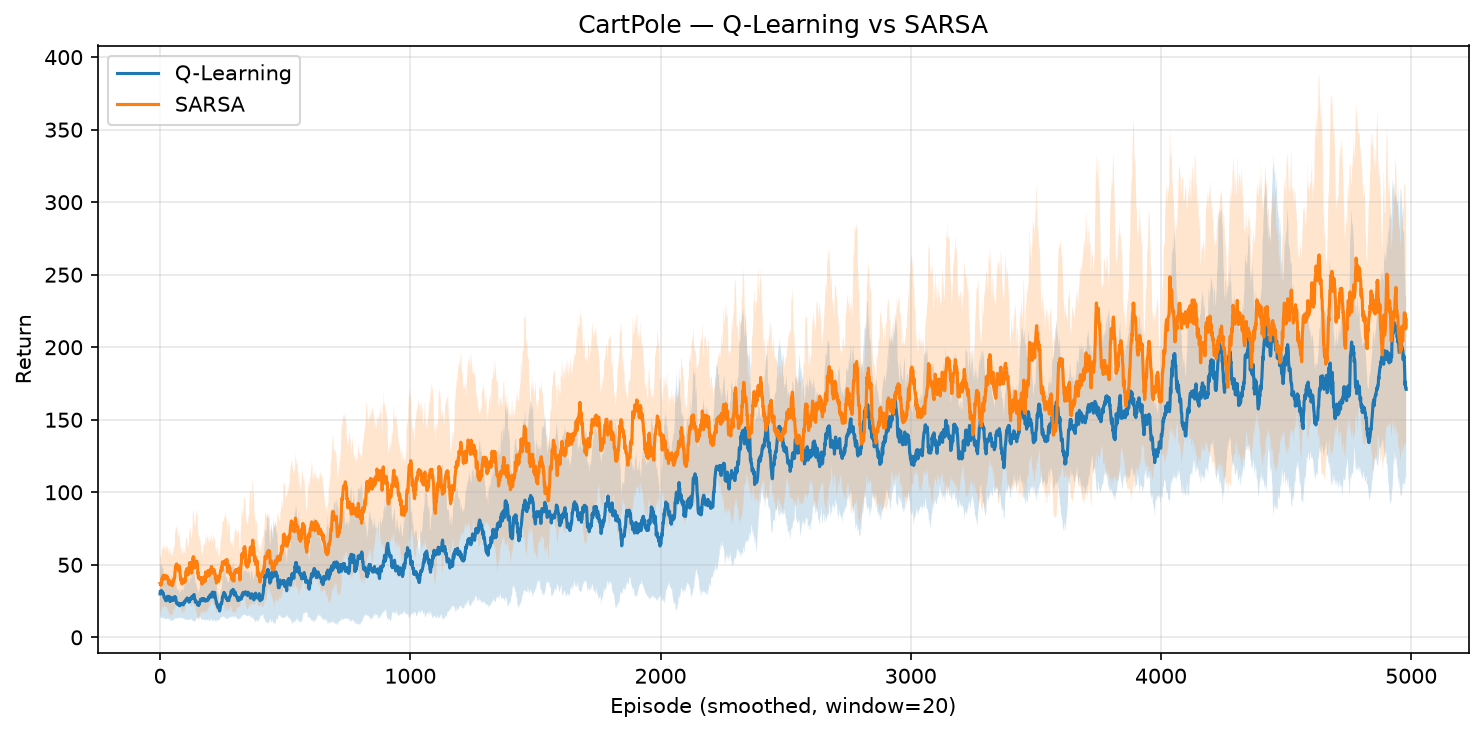
\includegraphics[width=0.55\linewidth]{cartpole_control_comparison.png}
\caption{CartPole: Q\hbox{-}Learning vs SARSA a parit\`a di iperparametri (media su 3
seed, banda $\pm1\sigma$). SARSA (arancio) sta sopra per tutto il training; entrambe le
curve salgono ancora a 10\,000 episodi.}
\label{fig:cp-control}
\end{figure}

\begin{table}[htbp]
\centering
\caption{CartPole, controllo: Q-Learning vs SARSA a parit\`a di iperparametri ($\alpha=0.1$, $\gamma=0.99$, $\varepsilon=0.1$), media su 3 seed. Il return massimo dell'ambiente \`e 500; entrambe le curve sono ancora in salita a fine budget.}
\label{tab:cartpole-control}
\begin{tabular}{lccc}
\toprule
Algoritmo & Return iniziale & Return finale & Episodi/seed \\
          & (primi 100 ep) & (ultimo 10\% ep, media $\pm$ std) & \\
\midrule
Q-Learning & 26.6 & $223.6 \pm 49.4$ & 10000 \\
SARSA & 40.8 & $258.3 \pm 31.1$ & 10000 \\
\bottomrule
\end{tabular}
\end{table}


% =====================================================================
\subsection{CartPole --- sensibilit\`a a $\varepsilon$, $\alpha$, $\gamma$}
\label{sec:res-cartpole-sens}

La Fig.~\ref{fig:cp-sens} riporta le sei sweep. Averle
fatte per \emph{entrambi} gli algoritmi non \`e ridondanza: su $\alpha$ i due si
comportano diversamente, ed \`e il dato pi\`u interessante della sezione.

\begin{itemize}
  \item \textbf{$\gamma$ --- l'effetto pi\`u netto.} Valori alti vincono per entrambi:
        $\gamma \in \{0.99, 1.0\}$ arriva a $230$--$280$, $\gamma \in \{0.9, 0.95\}$ si
        blocca a $140$--$165$. Strutturale: CartPole \`e un compito di
        \emph{sopravvivenza} con reward $+1$/passo, quindi il valore di uno stato
        \emph{\`e} quanto a lungo si sopravvive. Con $\gamma=0.9$ l'orizzonte effettivo
        \`e $\approx 1/(1-\gamma) = 10$ passi: l'agente non pu\`o vedere la caduta che
        sta preparando.
  \item \textbf{$\varepsilon$ --- serve, ma il troppo non nuoce.} $\varepsilon=0.01$ \`e
        il peggiore per entrambi ($105$--$130$), mentre $\varepsilon=0.3$ \emph{non}
        degrada ($220$--$250$, come $0.1$): il reward denso perdona l'esplorazione,
        perch\'e una mossa casuale costa al pi\`u qualche passo. Su Acrobot accadr\`a
        l'esatto contrario (Sez.~\ref{sec:res-acrobot-eps}): l'effetto di $\varepsilon$
        dipende dalla struttura del reward, non \`e una propriet\`a dell'algoritmo.
  \item \textbf{$\alpha$ --- qui i due divergono.} Per Q\hbox{-}Learning $\alpha=0.5$ e
        $\alpha=0.1$ finiscono appaiati ($200$--$220$), con $0.5$ pi\`u veloce
        all'inizio. Per \emph{SARSA} invece $\alpha=0.5$ parte forte ma
        \textbf{satura sotto} $\alpha=0.1$ ($\approx 210$ contro $\approx 260$). SARSA
        \`e on-policy, quindi il target $Q(S',A')$ contiene la casualit\`a dell'azione
        $A'$: un $\alpha$ alto insegue quel rumore invece di mediarlo.
        Q\hbox{-}Learning, che usa il $\max$ (deterministico dato $Q$), ne soffre meno.
        $\alpha=0.01$ \`e troppo lento per entrambi ($45$--$95$).
\end{itemize}

\begin{figure}[htbp]
\centering
\begin{subfigure}{0.31\linewidth}
  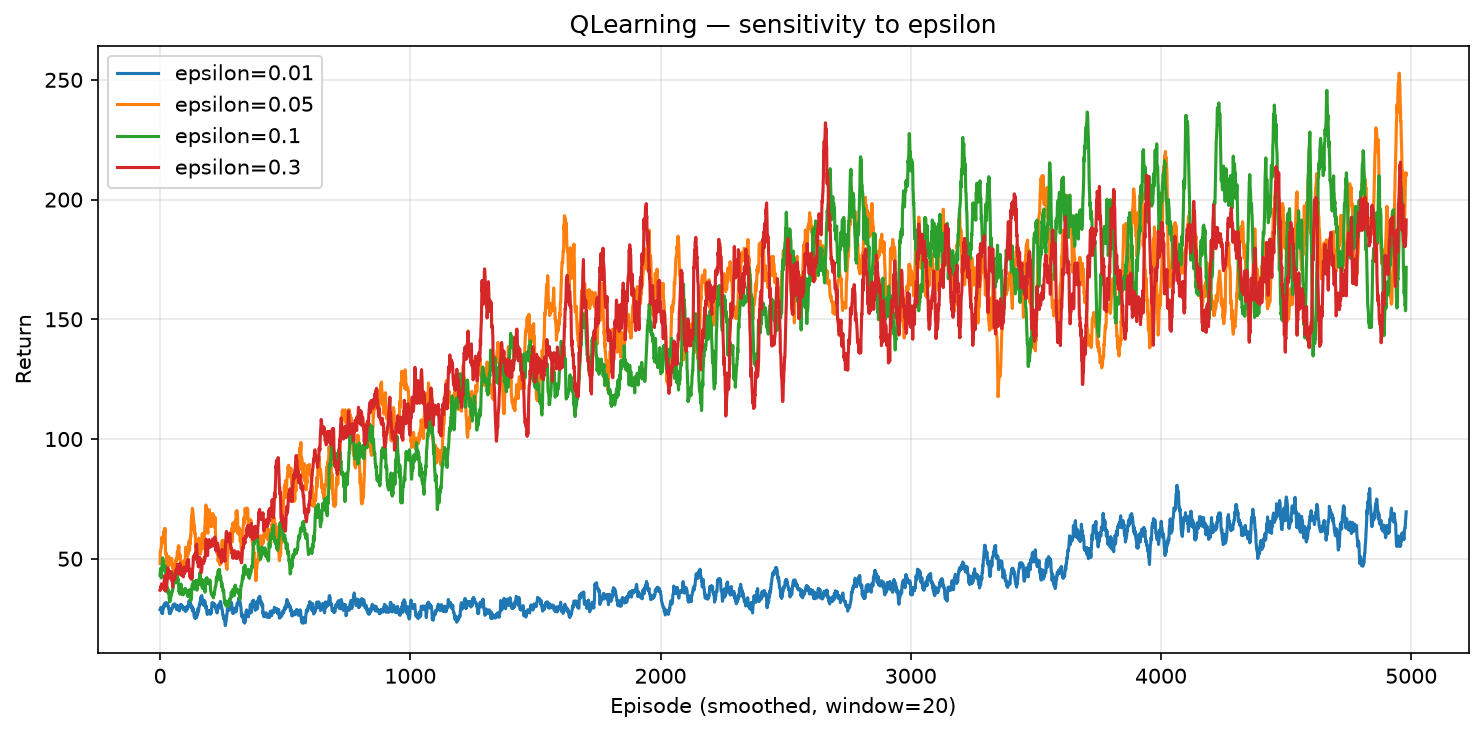
\includegraphics[width=\linewidth]{cartpole_sensitivity_QLearning_epsilon.png}
  \caption{Q-Learning, $\varepsilon$}
\end{subfigure}\hfill
\begin{subfigure}{0.31\linewidth}
  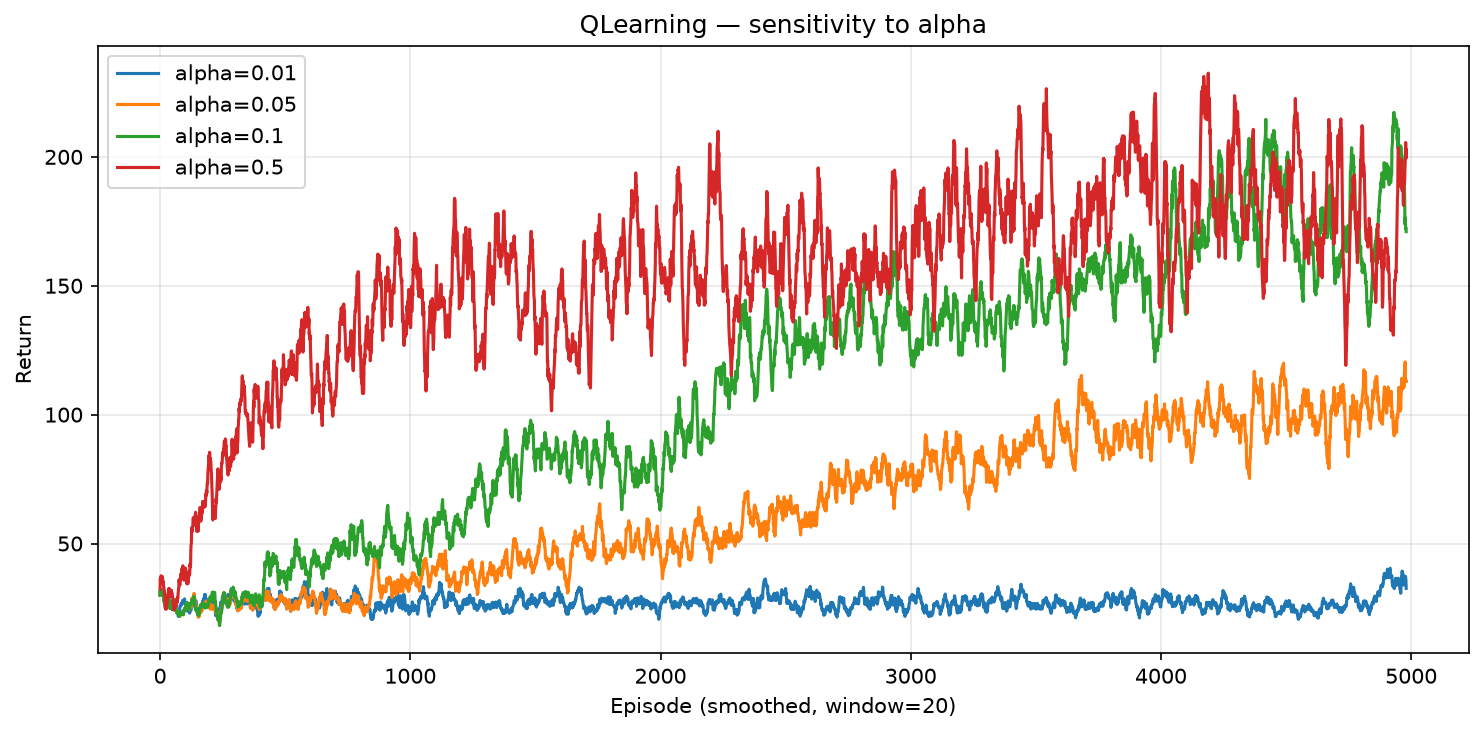
\includegraphics[width=\linewidth]{cartpole_sensitivity_QLearning_alpha.png}
  \caption{Q-Learning, $\alpha$}
\end{subfigure}\hfill
\begin{subfigure}{0.31\linewidth}
  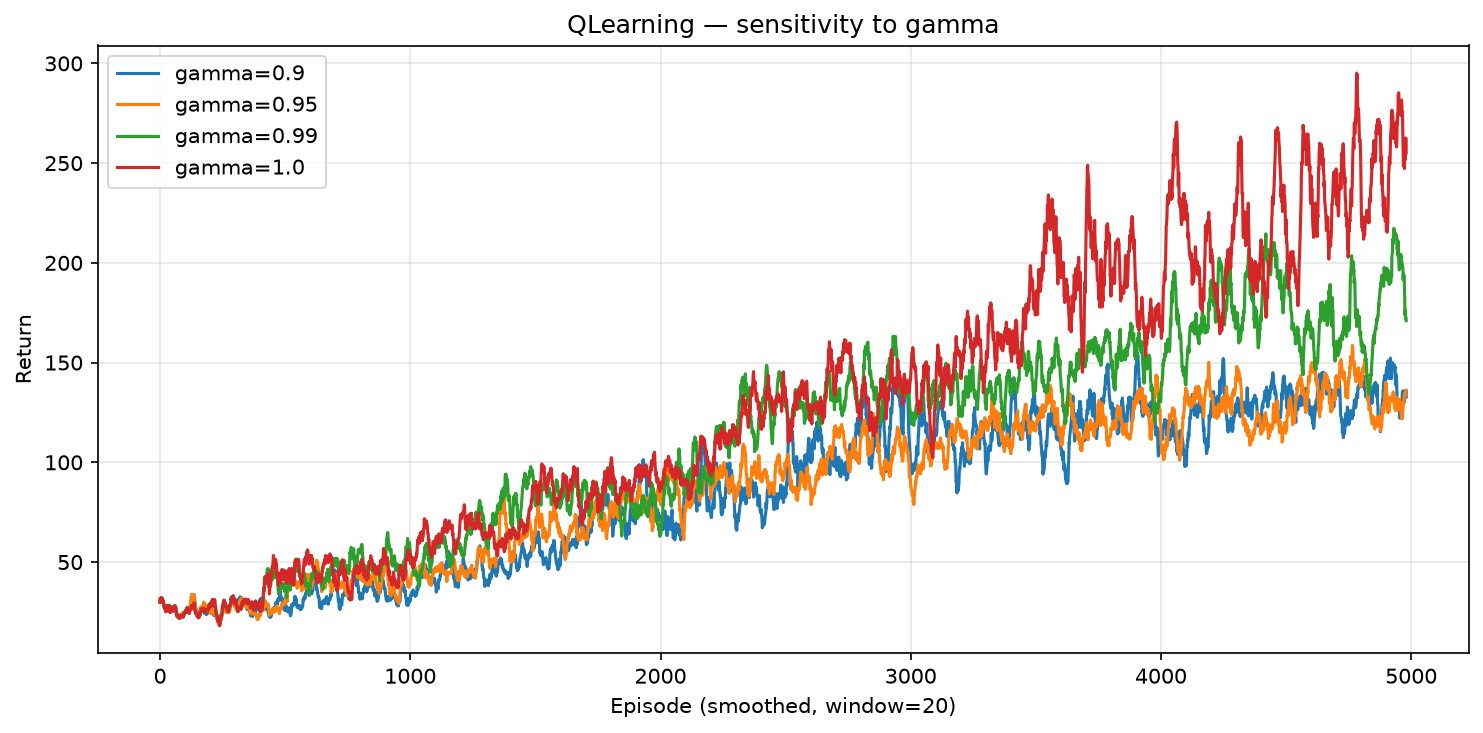
\includegraphics[width=\linewidth]{cartpole_sensitivity_QLearning_gamma.png}
  \caption{Q-Learning, $\gamma$}
\end{subfigure}

\medskip
\begin{subfigure}{0.31\linewidth}
  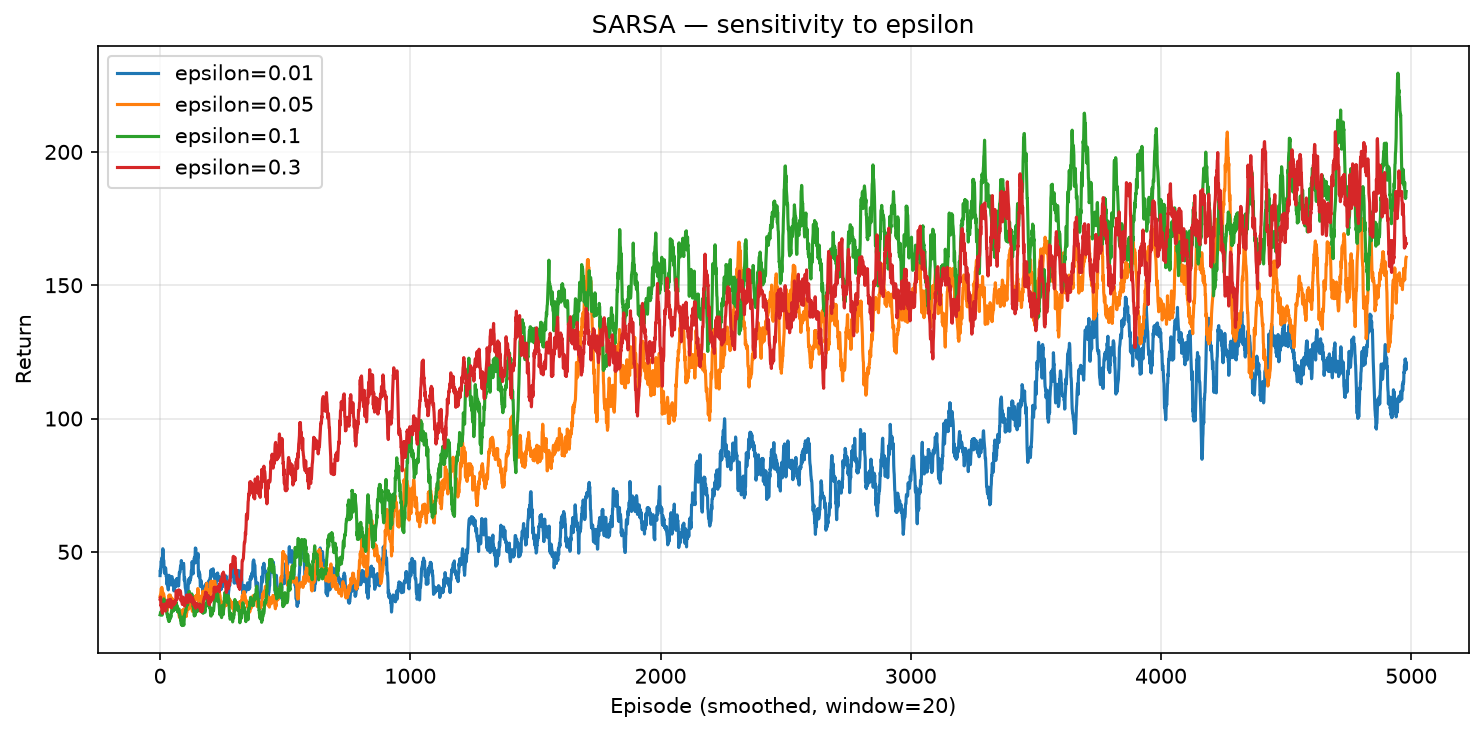
\includegraphics[width=\linewidth]{cartpole_sensitivity_SARSA_epsilon.png}
  \caption{SARSA, $\varepsilon$}
\end{subfigure}\hfill
\begin{subfigure}{0.31\linewidth}
  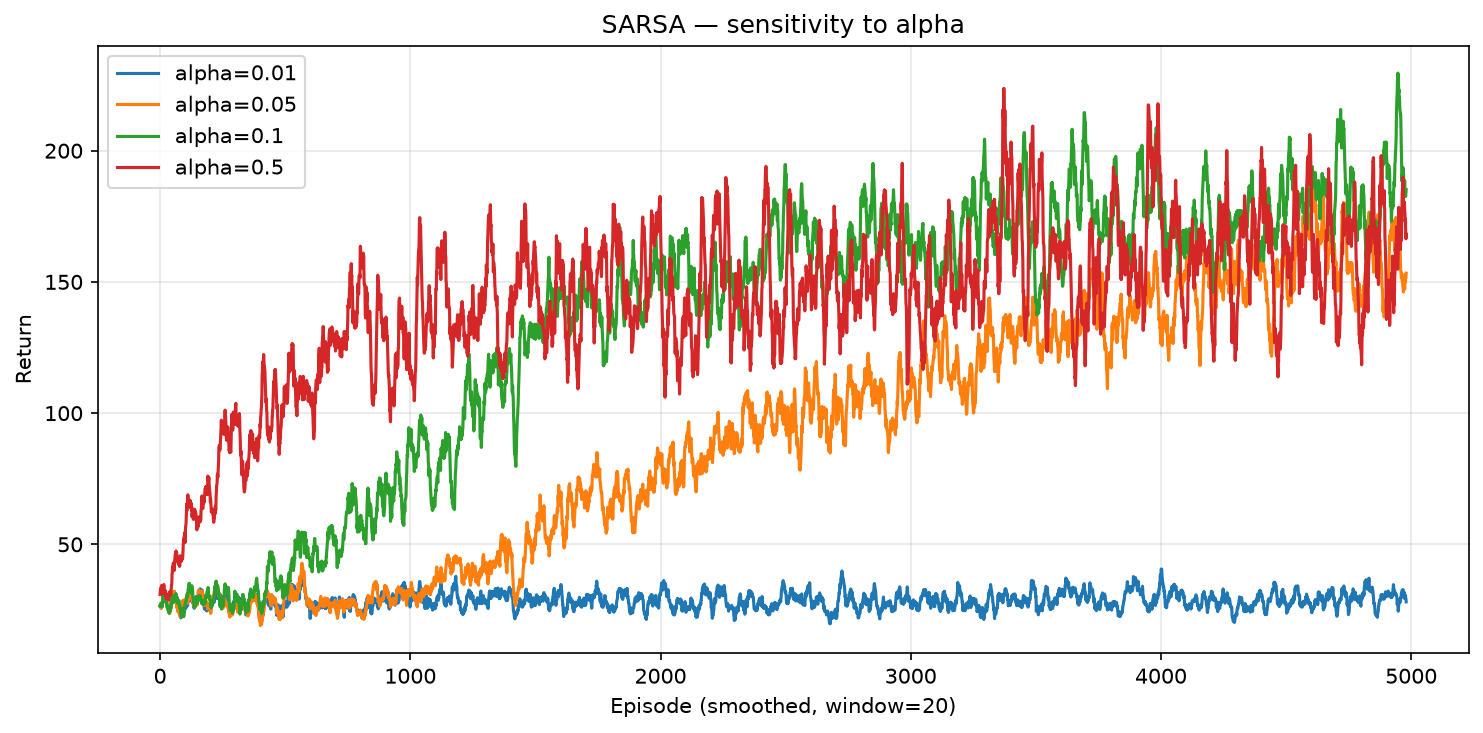
\includegraphics[width=\linewidth]{cartpole_sensitivity_SARSA_alpha.png}
  \caption{SARSA, $\alpha$}
\end{subfigure}\hfill
\begin{subfigure}{0.31\linewidth}
  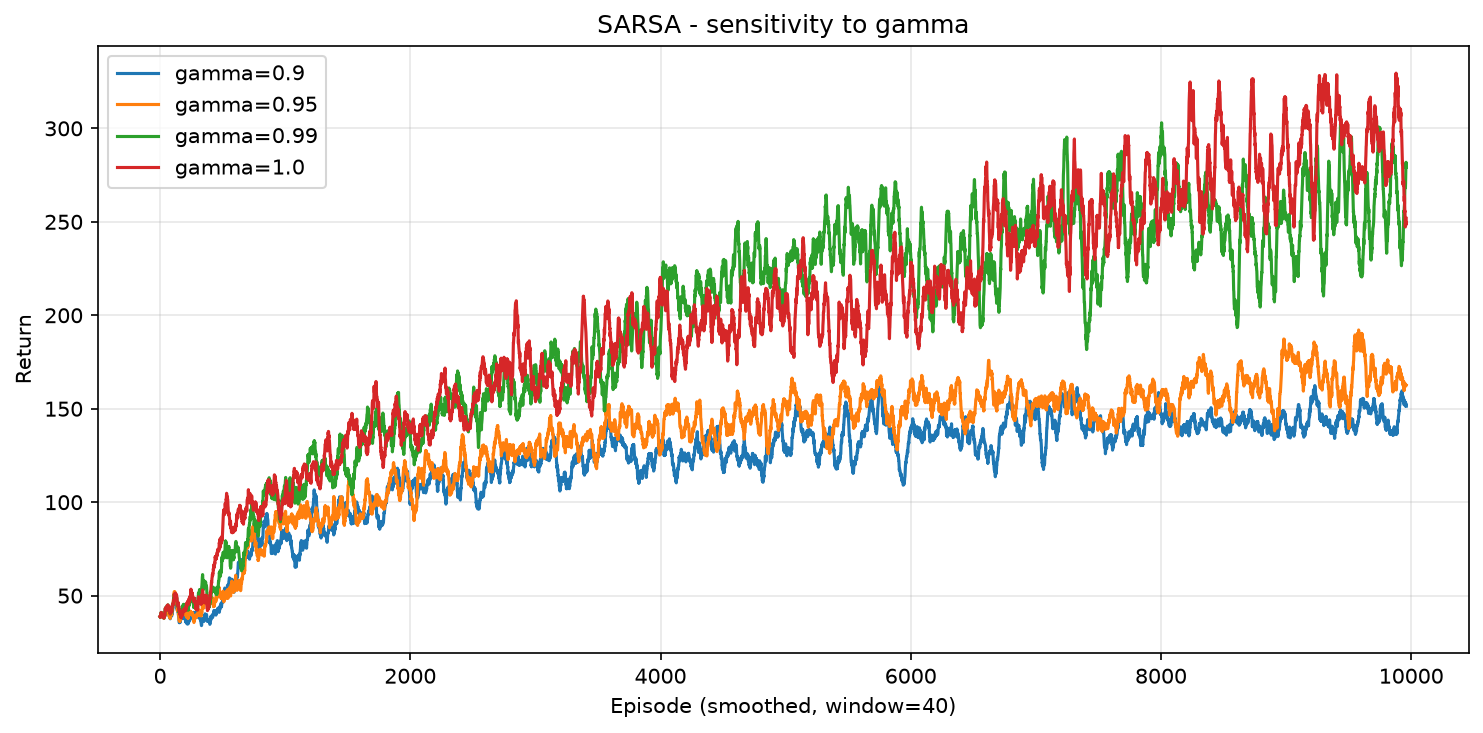
\includegraphics[width=\linewidth]{cartpole_sensitivity_SARSA_gamma.png}
  \caption{SARSA, $\gamma$}
\end{subfigure}
\caption{CartPole: le sei sweep di sensibilit\`a (media su 3 seed; bande omesse per
leggibilit\`a, Sez.~\ref{sec:experiments-reading}). Riga superiore Q\hbox{-}Learning,
inferiore SARSA. $\gamma$ alto domina in entrambi; $\varepsilon$ troppo basso \`e il vero
problema, mentre $\varepsilon=0.3$ non danneggia. La differenza tra i due algoritmi sta
nel pannello $\alpha$: per SARSA (e) $\alpha=0.5$ (rosso) parte veloce ma satura
\emph{sotto} $\alpha=0.1$ (verde), mentre per Q\hbox{-}Learning (b) i due si equivalgono.}
\label{fig:cp-sens}
\end{figure}

% =====================================================================
\subsection{CartPole --- $\varepsilon$ costante vs annealing}
\label{sec:res-cartpole-anneal}

Mi aspettavo che l'annealing servisse a poco su CartPole, che ha reward denso e non \`e
limitato dall'esplorazione. Il beneficio c'\`e, ma \`e soprattutto sulla
\emph{stabilit\`a}: l'annealing ($1.0 \to 0.01$) chiude a \res{243.8}{23.9} contro
\res{223.6}{49.4} del costante (Fig.~\ref{fig:cp-anneal}). Il guadagno in media \`e
modesto ($+20$), ma la dispersione tra seed si \emph{dimezza}: ridurre $\varepsilon$ a
fine training toglie il rumore che la policy si porta dietro, e l'esito dipende meno dal
seed. Il prezzo \`e un avvio pi\`u lento, fino a $\approx 3500$ episodi.

\begin{figure}[htbp]
\centering
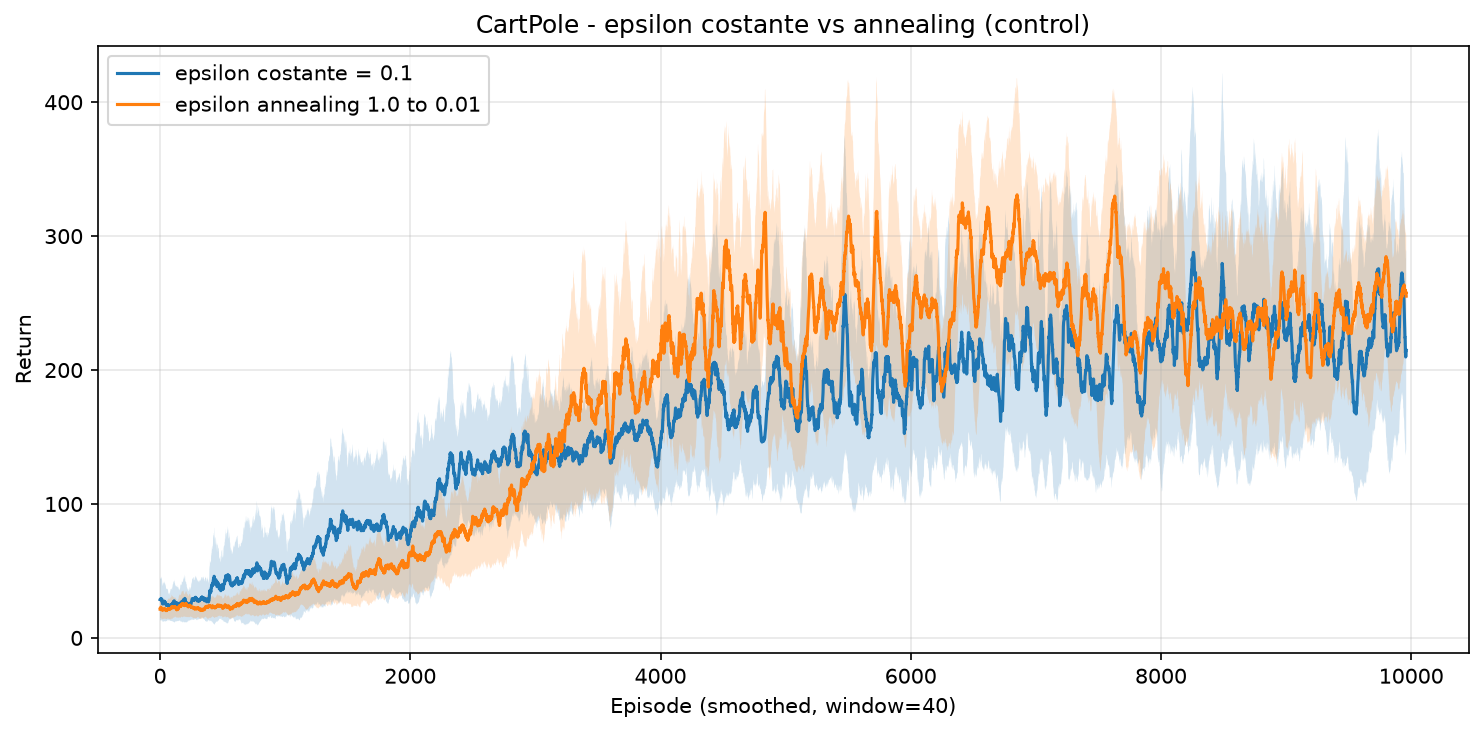
\includegraphics[width=0.55\linewidth]{cartpole_epsilon_annealing.png}
\caption{CartPole: $\varepsilon$ costante $=0.1$ vs annealing $1.0 \to 0.01$.
L'annealing paga un avvio pi\`u lento, poi sorpassa e chiude con banda $\pm1\sigma$
visibilmente pi\`u stretta.}
\label{fig:cp-anneal}
\end{figure}

% =====================================================================
\subsection{CartPole --- MC vs TD(0): bias, varianza, stabilit\`a}
\label{sec:res-cartpole-pred}

\textbf{Il return non pu\`o distinguere i due stimatori} (Fig.~\ref{fig:cp-pred}a): le
curve sono \emph{identiche per costruzione}, perch\'e MC e TD(0) valutano la
\emph{stessa} policy fissa e generano quindi gli stessi episodi (return $\approx 330$).
La curva di MC \`e letteralmente nascosta sotto quella di TD. Non \`e un errore di
plotting: \`e la prova che la differenza tra i due metodi non vive nel return ma nelle
stime $V(s)$. Per inciso, quei $\approx 330$ passi sono ottenuti dalla policy greedy
\emph{senza} esplorazione, contro i $\approx 224$ della curva di training: gran parte
del divario dal massimo \`e il costo di $\varepsilon$, non incapacit\`a della policy.

\textbf{La differenza vive nelle stime} (Fig.~\ref{fig:cp-pred}b), ed \`e il quadro
classico di S\&B \S6.2. \textbf{MC} salta al valore corretto ($81.07 \pm 0.17$) in poche
decine di episodi ma con un picco iniziale violento: \`e \emph{non distorto} e ad
\emph{alta varianza}, perch\'e ogni aggiornamento usa il return completo di una
traiettoria di $\approx 330$ passi. \textbf{TD(0)} parte da 0 e sale lentamente e in modo
liscio, fermandosi a $70.50 \pm 0.28$ dopo 6000 episodi --- ancora $13\%$ sotto MC: \`e
\emph{distorto} (fa bootstrap su una stima ancora sbagliata) ma a \emph{bassa varianza}.

\textbf{Il bias di TD(0) non \`e una costante: dipende dalla policy valutata.} \`E il
risultato che giustifica l'aver valutato anche la policy casuale
(Fig.~\ref{fig:cp-pred-random}). L\`i gli episodi durano $\approx 22$ passi, lo stato di
riferimento \`e vicinissimo alla terminazione, e TD(0) \emph{raggiunge} MC entro
$\approx 5000$ episodi ($17.04$ contro $17.43$): il bias sparisce. Con la policy appresa
gli episodi sono quindici volte pi\`u lunghi e il bootstrap deve propagare il valore un
passo alla volta. La distorsione di TD(0) \`e quindi una funzione della \emph{distanza
temporale} tra lo stato e il reward, non un difetto fisso dell'algoritmo.

\begin{figure}[htbp]
\centering
\begin{subfigure}{0.46\linewidth}
  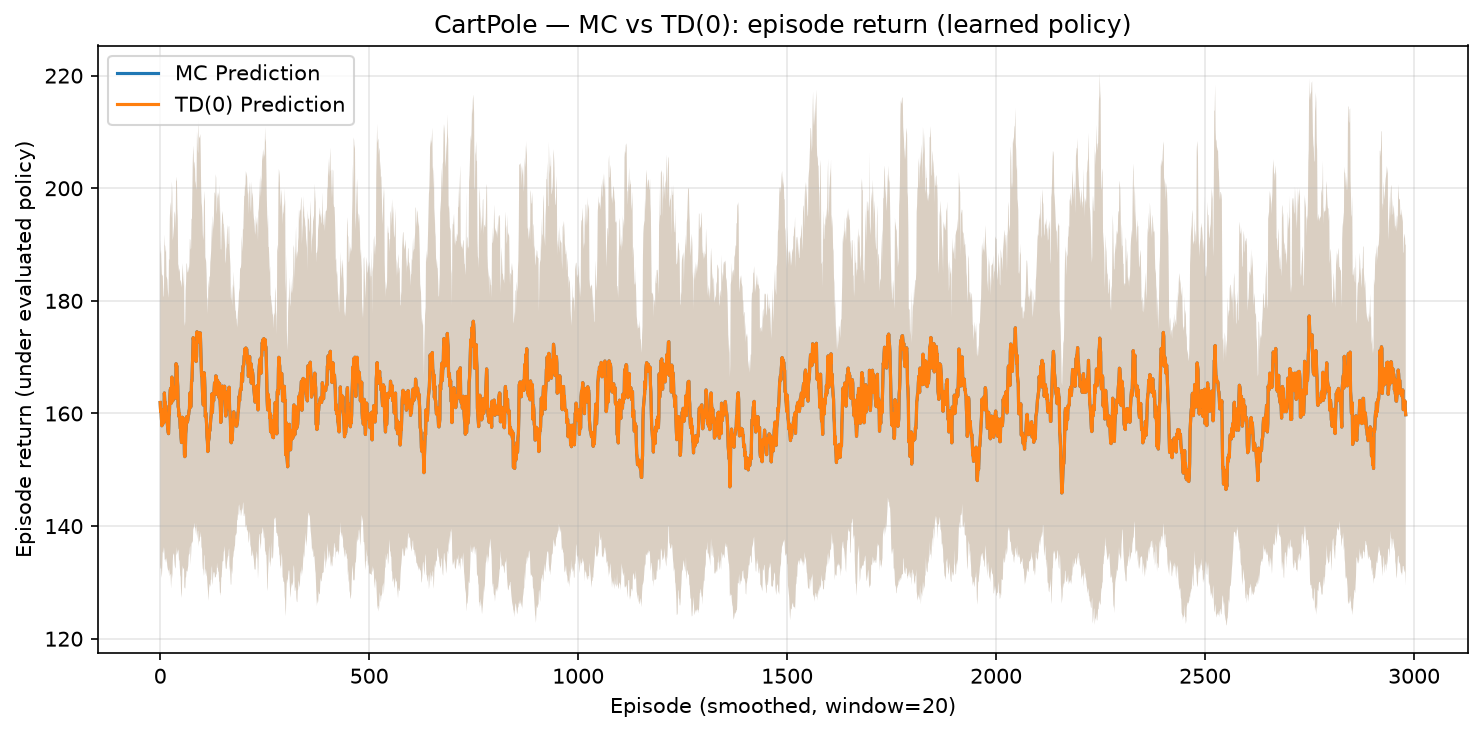
\includegraphics[width=\linewidth]{cartpole_prediction_learned_return.png}
  \caption{Return: identico per costruzione.}
\end{subfigure}\hfill
\begin{subfigure}{0.46\linewidth}
  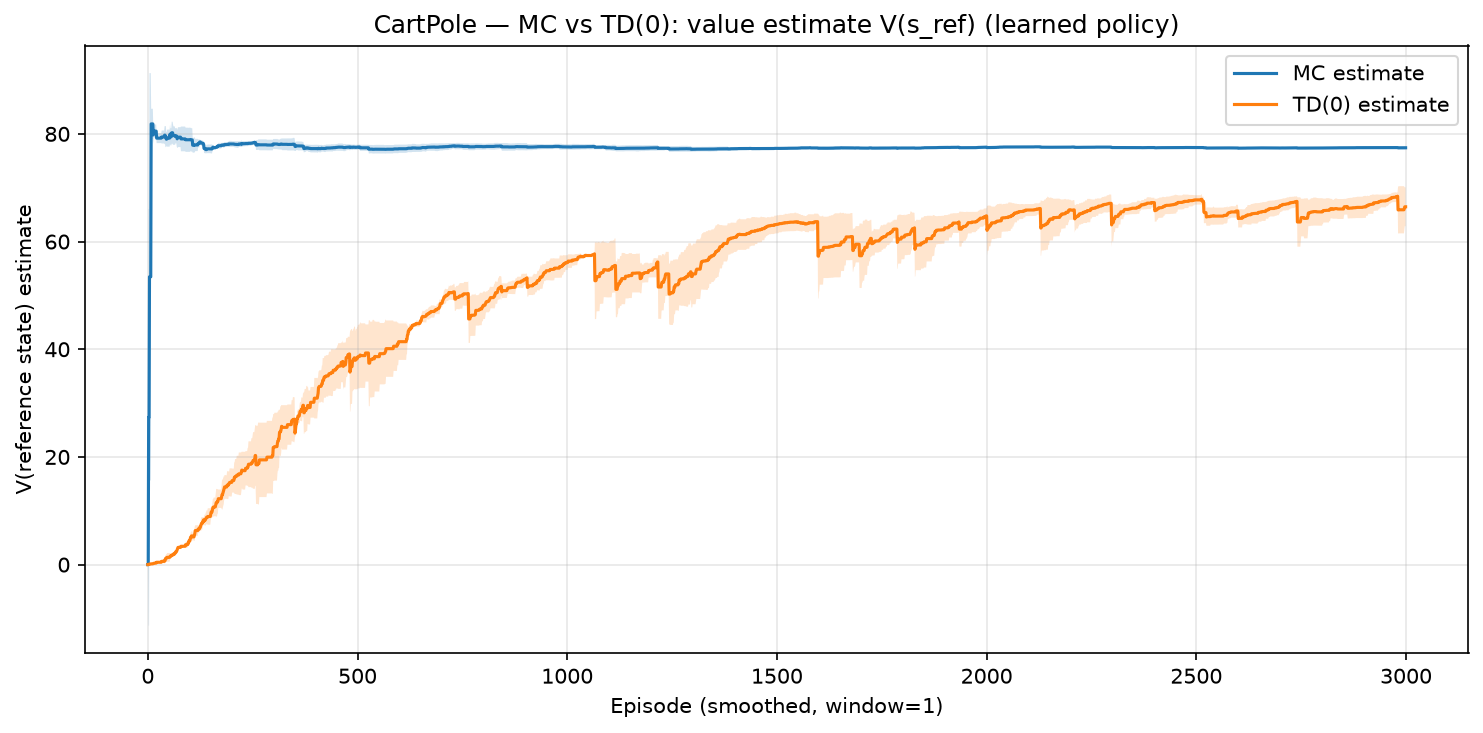
\includegraphics[width=\linewidth]{cartpole_prediction_learned_value.png}
  \caption{Stima $V(s_{\text{ref}})$: qui divergono.}
\end{subfigure}
\caption{CartPole, MC vs TD(0) sulla \textbf{policy appresa}. (a) Stessa policy, stessi
episodi: il return non pu\`o dire nulla sugli stimatori. (b) Le stime invece raccontano
tutto: MC (blu) non distorto e ad alta varianza iniziale, TD(0) (arancio) liscio ma
distorto verso l'inizializzazione e non ancora convergente a 6000 episodi.}
\label{fig:cp-pred}
\end{figure}

\begin{figure}[htbp]
\centering
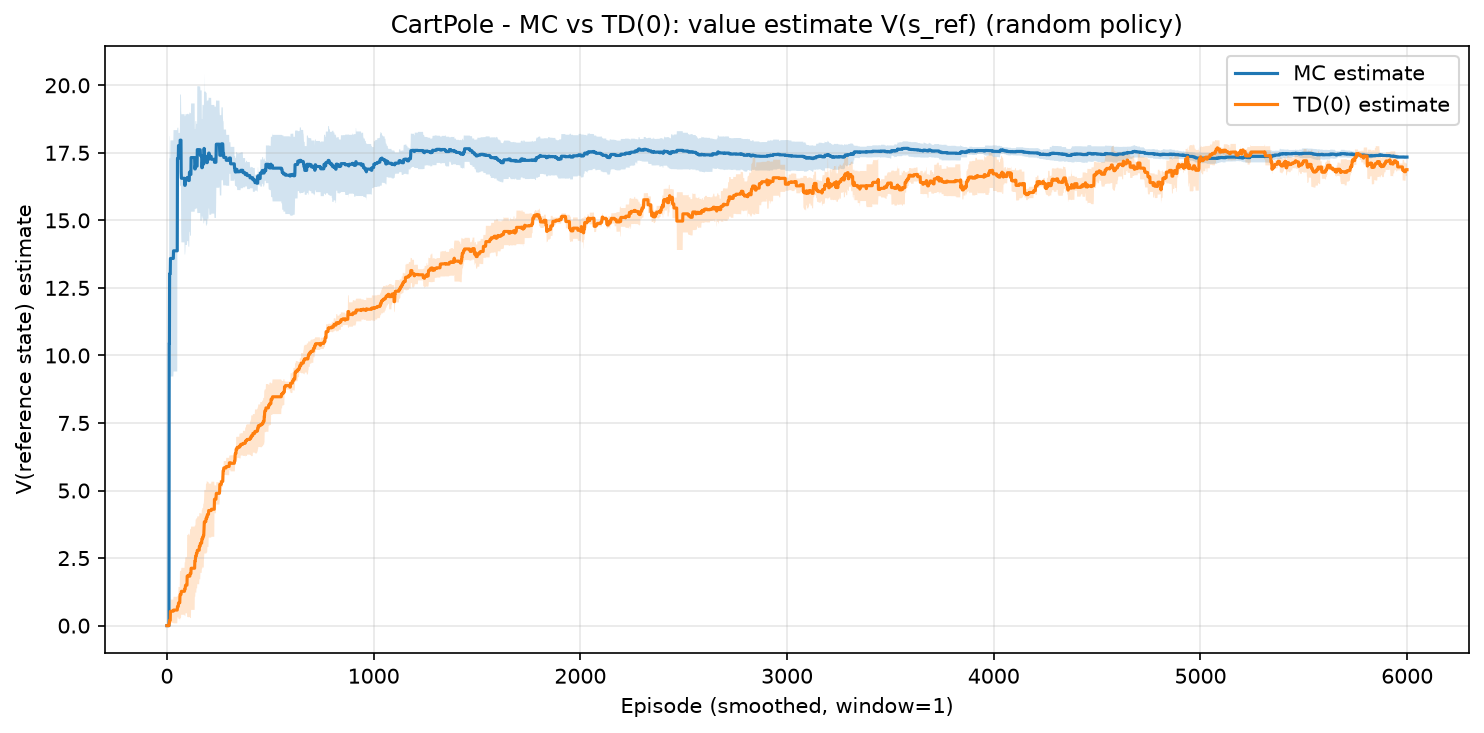
\includegraphics[width=0.52\linewidth]{cartpole_prediction_random_value.png}
\caption{CartPole, MC vs TD(0) sulla \textbf{policy casuale}. Con episodi corti
($\approx 22$ passi) il bootstrap propaga in fretta e TD \emph{raggiunge} MC: il bias
dipende da quanto lo stato \`e lontano dalla terminazione. Da confrontare con la
Fig.~\ref{fig:cp-pred}b.}
\label{fig:cp-pred-random}
\end{figure}

Le figure del return sulla policy casuale e su Acrobot esistono in \code{figures/} ma
non sono riportate: mostrano lo stesso fenomeno di Fig.~\ref{fig:cp-pred}a (curve
sovrapposte per costruzione) e non aggiungono informazione.

% =====================================================================
\subsection{Acrobot --- controllo}
\label{sec:res-acrobot-control}

Entrambi gli algoritmi migliorano da $\approx -470$ (vicino al casuale, $-500$) fino a
\res{-341.4}{27.8} (Q\hbox{-}Learning) e \res{-348.6}{3.2} (SARSA), restando lontanissimi
dall'ottimo ($\approx -100$): l'agente impara qualche spinta utile, non uno swing-up
efficiente (Fig.~\ref{fig:ac-control}, Tab.~\ref{tab:acrobot-control}).

Il dato pi\`u istruttivo \`e la \textbf{forma} della curva: il grosso del miglioramento
avviene entro i primi $\approx 5000$ episodi, poi le curve oscillano attorno a
$-340/-350$ \emph{senza migliorare} per altri 15\,000. Non \`e lentezza, \`e un tetto:
raddoppiare il budget non lo sposta. Con 46\,656 stati e un reward informativo solo
quando l'obiettivo viene raggiunto per caso, la Q-table a 6 bin non ha la risoluzione per
rappresentare una politica migliore --- ipotesi che la sezione seguente verifica.

Notevole l'inversione rispetto a CartPole sulla varianza: qui \`e \textbf{SARSA} ad
essere drasticamente pi\`u stabile ($\pm 3.2$ contro $\pm 27.8$). La stabilit\`a relativa
dei due algoritmi non \`e una loro propriet\`a intrinseca ma dipende dall'ambiente; la
Sez.~\ref{sec:discussion} riprende il punto.

\begin{figure}[htbp]
\centering
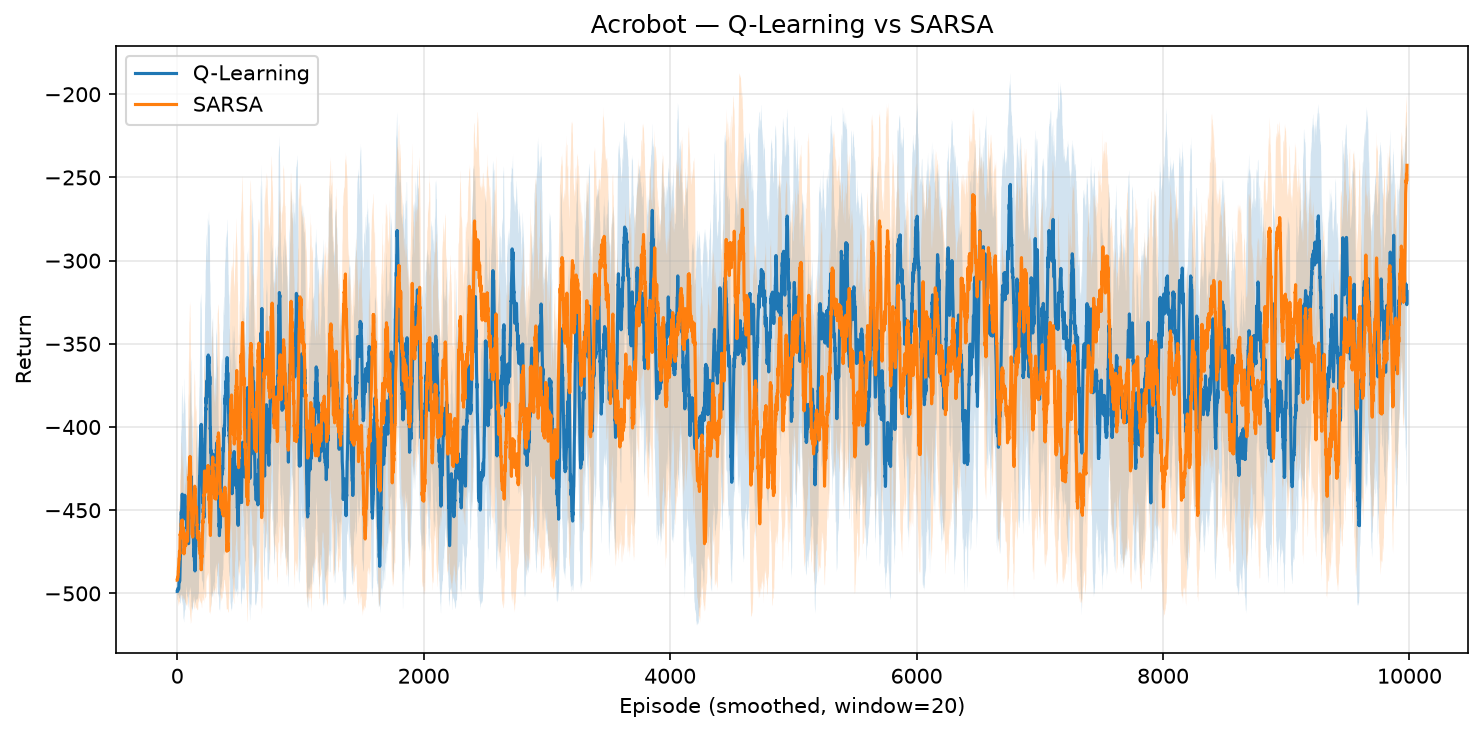
\includegraphics[width=0.55\linewidth]{acrobot_control_comparison.png}
\caption{Acrobot: Q\hbox{-}Learning vs SARSA. Miglioramento reale rispetto al casuale
($-500$), ma plateau precoce ($\approx 5000$ episodi) e molto lontano dall'ottimo
($\approx -100$).}
\label{fig:ac-control}
\end{figure}

\begin{table}[htbp]
\centering
\caption{Acrobot, controllo: Q-Learning vs SARSA, media su 3 seed. Policy casuale $\approx -500$; un buon swing-up raggiunge $\approx -100$.}
\label{tab:acrobot-control}
\begin{tabular}{lccc}
\toprule
Algoritmo & Return iniziale & Return finale & Episodi/seed \\
          & (primi 100 ep) & (ultimo 10\% ep, media $\pm$ std) & \\
\midrule
Q-Learning & -468.0 & $-341.4 \pm 27.8$ & 20000 \\
SARSA & -473.2 & $-348.6 \pm 3.2$ & 20000 \\
\bottomrule
\end{tabular}
\end{table}


% =====================================================================
\subsection{Acrobot --- risoluzione della discretizzazione}
\label{sec:res-acrobot-bins}

\textbf{\`E l'esperimento che ha smentito la mia ipotesi di partenza}, ed \`e il
risultato pi\`u istruttivo del progetto. L'ipotesi: aumentare i bin \emph{peggiora}
l'apprendimento, perch\'e lo spazio cresce come $\text{bin}^6$ e a 10 bin ($10^6$ stati)
la tabella diventa irrimediabilmente sparsa --- la curse of dimensionality da manuale.

I dati dicono l'\textbf{opposto}, in modo monotono e non ambiguo
(Fig.~\ref{fig:ac-bins}): a 20\,000 episodi \textbf{10 bin \`e la configurazione
migliore} ($\approx -280$) e \textbf{4 bin la peggiore} ($\approx -430$), con 8 e 6
ordinatamente in mezzo.

Avevo confrontato il costo sbagliato. Le dinamiche di Acrobot richiedono
\emph{precisione angolare}: con 4 bin per dimensione, configurazioni del pendolo che
richiedono coppie \emph{opposte} finiscono nello \emph{stesso} stato discreto. La
Q-table non pu\`o rappresentare politiche diverse per stati che non sa distinguere, e
nessun numero di episodi lo ripara --- infatti la curva a 4 bin resta piatta e rumorosa
fino in fondo. Questo costo di \emph{aliasing} domina quello della sparsit\`a: la curse
of dimensionality \`e reale in principio, ma a questo budget non \`e ancora il vincolo
attivo. \`E anche la giustificazione empirica del passaggio al DQN: per avere insieme
precisione e generalizzazione serve un approssimatore di funzione.

\begin{figure}[htbp]
\centering
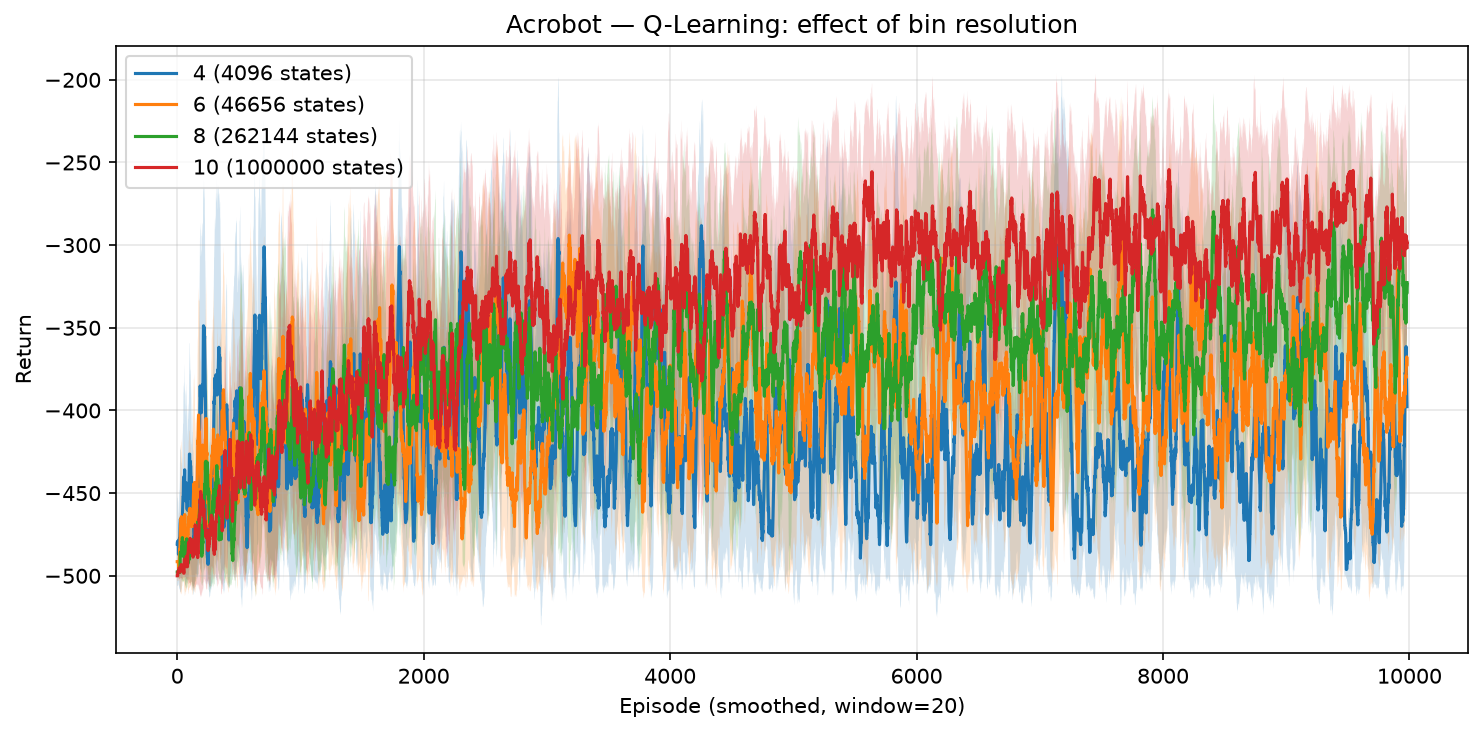
\includegraphics[width=0.55\linewidth]{acrobot_bin_resolution.png}
\caption{Acrobot: effetto della risoluzione di discretizzazione (Q\hbox{-}Learning,
20\,000 episodi). Contrariamente all'ipotesi, 10 bin ($10^6$ stati, rosso) \`e la
configurazione \emph{migliore} e 4 bin (blu) la peggiore, con ordinamento monotono: 4
bin non riescono a distinguere stati che richiedono coppie opposte.}
\label{fig:ac-bins}
\end{figure}

% =====================================================================
\subsection{Acrobot --- esplorazione: $\varepsilon$ costante e annealing}
\label{sec:res-acrobot-eps}

Anche qui l'attesa era chiara --- reward sparso $\Rightarrow$ serve \emph{pi\`u}
esplorazione --- e anche qui la sweep a $\varepsilon$ costante dice il contrario
(Fig.~\ref{fig:ac-explore}a): i valori \emph{bassi} vincono ($\varepsilon = 0.05$ arriva
a $\approx -310$) e $\varepsilon = 0.4$ \`e nettamente il peggiore ($\approx -450$), di
nuovo in ordine monotono.

Il punto non \`e che l'esplorazione sia inutile, ma che \textbf{l'esplorazione
\emph{costante} \`e lo strumento sbagliato}: con $\varepsilon = 0.4$ l'agente continua a
iniettare coppie casuali \emph{anche dopo} aver trovato uno swing-up, distruggendolo ad
ogni episodio.

L'annealing conferma la lettura e chiude il cerchio (Fig.~\ref{fig:ac-explore}b): lo
schedule $1.0 \to 0.01$ raggiunge \res{-316.3}{24.5} contro \res{-341.4}{27.8} del
miglior $\varepsilon$ costante --- il guadagno pi\`u grande ottenuto su Acrobot senza
toccare l'algoritmo. Il prezzo \`e visibile: per $\approx 5000$ episodi la curva annealed
\`e inchiodata a $-500$ (con $\varepsilon \approx 1$ l'agente \`e di fatto casuale),
sorpassa attorno a $9000$ e da l\`i resta sopra. Il confronto con CartPole, dove lo stesso
schedule d\`a un guadagno modesto, isola il meccanismo: l'annealing paga dove
l'esplorazione \`e davvero il collo di bottiglia.

\begin{figure}[htbp]
\centering
\begin{subfigure}{0.46\linewidth}
  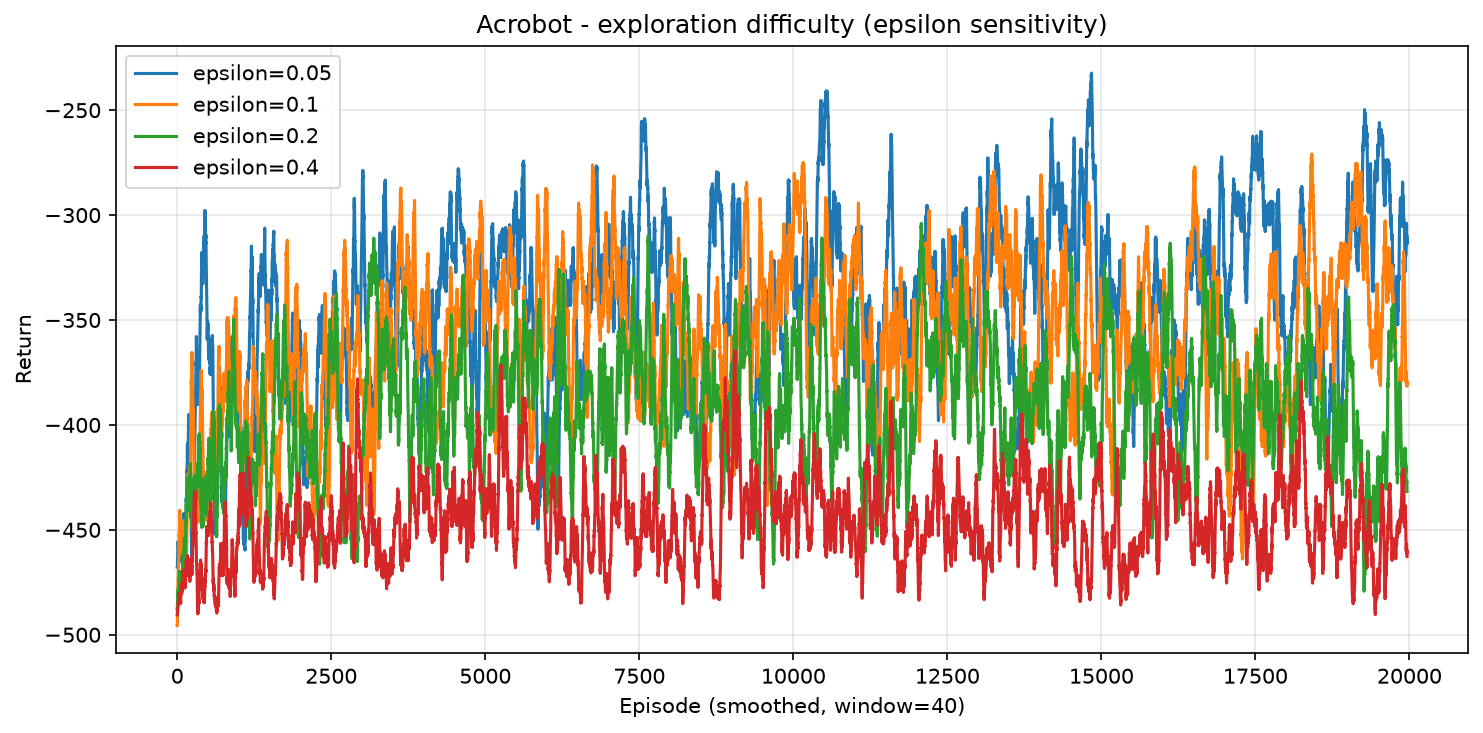
\includegraphics[width=\linewidth]{acrobot_sensitivity_epsilon.png}
  \caption{$\varepsilon$ costante: basso batte alto.}
\end{subfigure}\hfill
\begin{subfigure}{0.46\linewidth}
  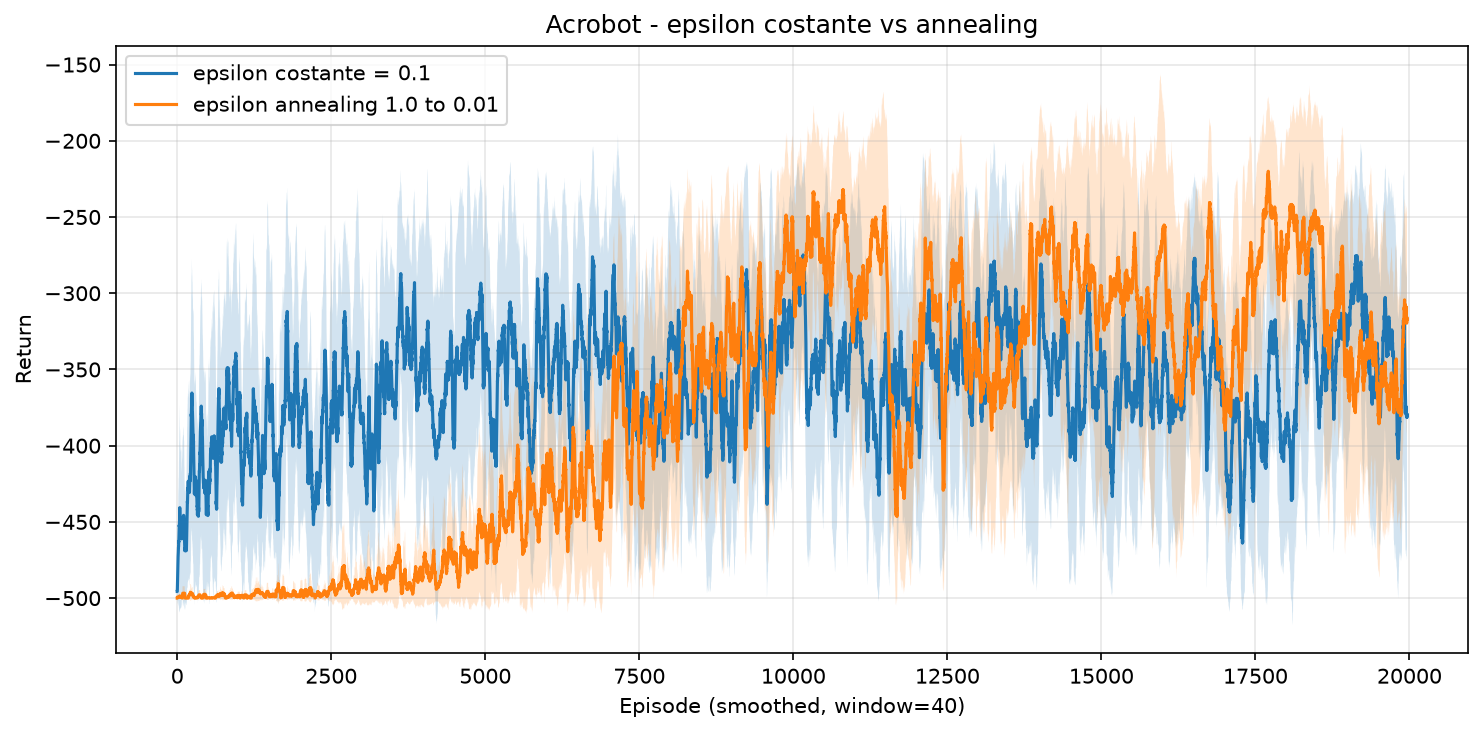
\includegraphics[width=\linewidth]{acrobot_epsilon_annealing.png}
  \caption{Annealing $1.0 \to 0.01$ vs costante $0.1$.}
\end{subfigure}
\caption{Acrobot, esplorazione. (a) A $\varepsilon$ \emph{costante} i valori bassi
vincono: un $\varepsilon$ alto tenuto fisso continua a distruggere lo swing-up appreso.
(b) Ma l'esplorazione \emph{decrescente} \`e la scelta giusta: paga $\approx 5000$
episodi a $-500$ e poi supera stabilmente il miglior $\varepsilon$ costante. Insieme, i
due pannelli dicono che il problema non era ``quanta'' esplorazione, ma ``quando''.}
\label{fig:ac-explore}
\end{figure}

% =====================================================================
\subsection{Acrobot --- MC vs TD(0)}
\label{sec:res-acrobot-pred}

Il bias di TD(0) \`e qui ancora pi\`u marcato che su CartPole (Fig.~\ref{fig:ac-pred}),
e conferma l'interpretazione data sopra. MC converge quasi subito a $-91.17 \pm 0.27$;
TD(0) parte da 0, \emph{scende lentamente} e dopo 6000 episodi \`e solo a
$-62.00 \pm 0.03$. Lo stato di riferimento \`e a $\approx 90$ passi dall'obiettivo e TD
propaga il valore un passo per volta: per uno stato cos\`i distante dal reward il
bootstrap \`e lentissimo e la stima resta ancorata all'inizializzazione.

Si noti la banda: quella di TD(0) \`e cos\`i stretta da risultare invisibile
($\pm 0.03$), quella di MC \`e ampia nei primi episodi. \`E il compromesso bias/varianza
nella sua forma pi\`u pura: TD \`e molto \emph{preciso} nel dare la risposta
\emph{sbagliata}, e ci mette molto ad arrivare a quella giusta.

\begin{figure}[htbp]
\centering
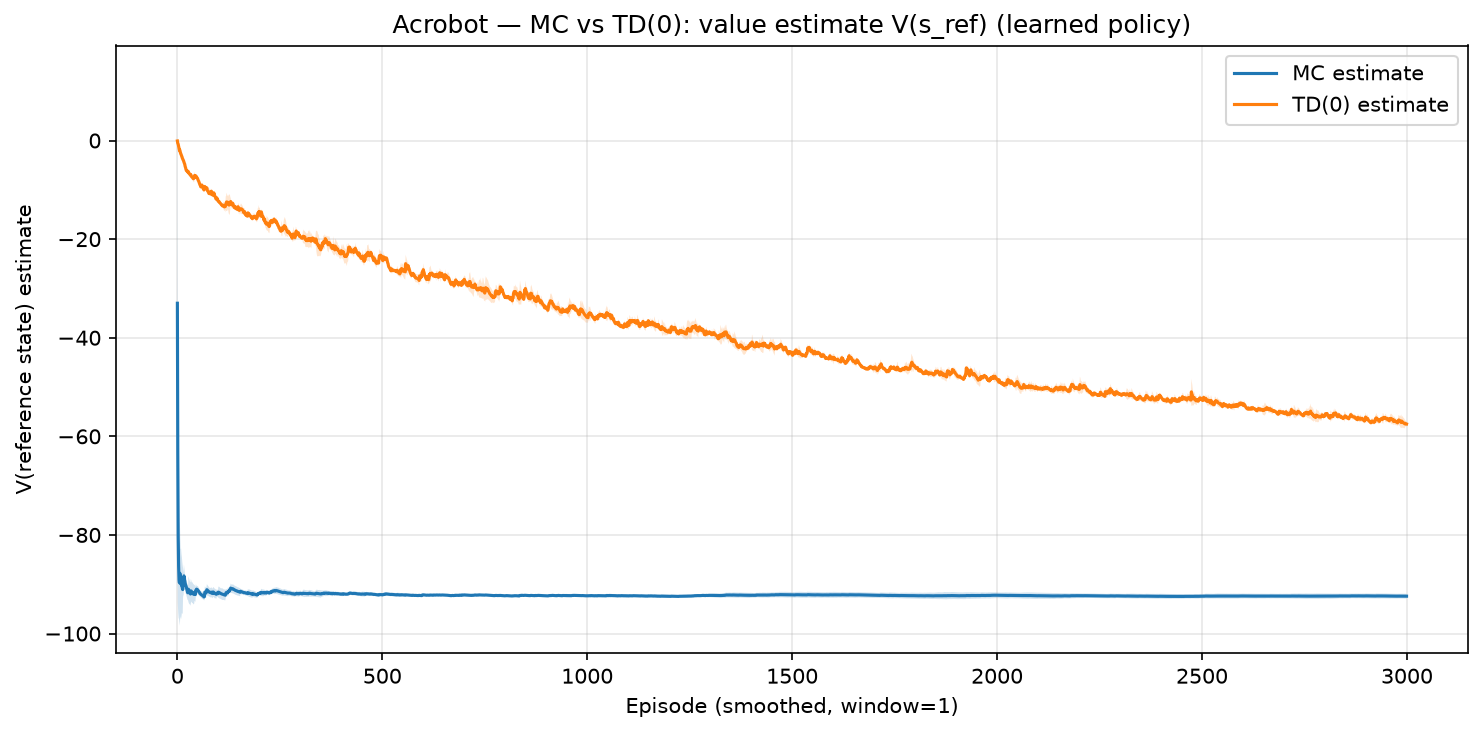
\includegraphics[width=0.54\linewidth]{acrobot_prediction_value.png}
\caption{Acrobot, MC vs TD(0): stima $V(s_{\text{ref}})$ della policy appresa. MC (blu)
converge subito a $\approx -91$; TD(0) (arancio) scende da 0 con estrema regolarit\`a ma
dopo 6000 episodi \`e ancora a $\approx -62$.}
\label{fig:ac-pred}
\end{figure}

% =====================================================================
\subsection{Pong --- ablazione del DQN}
\label{sec:res-pong}

Rispetto alla baseline casuale ($\approx -20.4$) e con soli 200k step
(Fig.~\ref{fig:pong-full}, Tab.~\ref{tab:pong-ablation}):
\begin{itemize}
  \item \textbf{DQN completo}: \res{-12.1}{0.9}. Apprende nettamente e in modo
        consistente tra i seed: il requisito della consegna (``mostrare apprendimento
        rispetto a policy casuale'') \`e soddisfatto con ampio margine.
  \item \textbf{Double DQN} (bonus): \res{-14.2}{0.8}. Apprende, con traiettoria simile
        al completo, senza superarlo.
  \item \textbf{Senza target network}: \res{-16.3}{2.8}. Apprende, ma pi\`u tardi e con
        varianza \emph{tripla}.
  \item \textbf{Senza replay} / \textbf{senza entrambi}: \res{-20.6}{0.2} e
        \res{-20.5}{0.3} --- \emph{nessun apprendimento}, restano al livello casuale.
\end{itemize}

\textbf{I due componenti non sono equivalenti} (Fig.~\ref{fig:pong-ablation}). Il
\emph{replay \`e indispensabile}: senza, la rete si addestra sul flusso di transizioni
consecutive fortemente correlate e in 200k step non impara nulla --- la curva \`e piatta.
La \emph{target network} \`e invece un \emph{acceleratore e stabilizzatore}: senza,
l'agente impara comunque (da $-20.4$ a $-16.3$), ma pi\`u tardi e con varianza tra seed
molto maggiore, il sintomo atteso del ``bersaglio mobile'' (ogni passo di gradiente
sposta anche il target). La distinzione tra componente \emph{necessario} e componente
\emph{utile} \`e il contenuto informativo dell'ablazione.

Un segnale indiretto ma elegante: il DQN completo produce \emph{meno} episodi per seed
($134$) delle configurazioni fallite ($\approx 240$). A parit\`a di step, un agente che
impara tiene in vita gli scambi pi\`u a lungo e gioca quindi meno partite: il numero di
episodi \`e esso stesso una misura di apprendimento.

Sul \textbf{Double DQN}: non supera il DQN base, ed \`e un esito spiegabile. Corregge la
\emph{sovrastima} dovuta al $\max$ su stime rumorose, un problema che si accumula su
orizzonti lunghi; a 200k step (lo $0.4\%$ del budget Nature) non ha ancora avuto tempo
di fare danno. Il bonus \`e implementato e funzionante --- semplicemente, in questo
regime, non c'\`e il male che dovrebbe curare.

\begin{figure}[htbp]
\centering
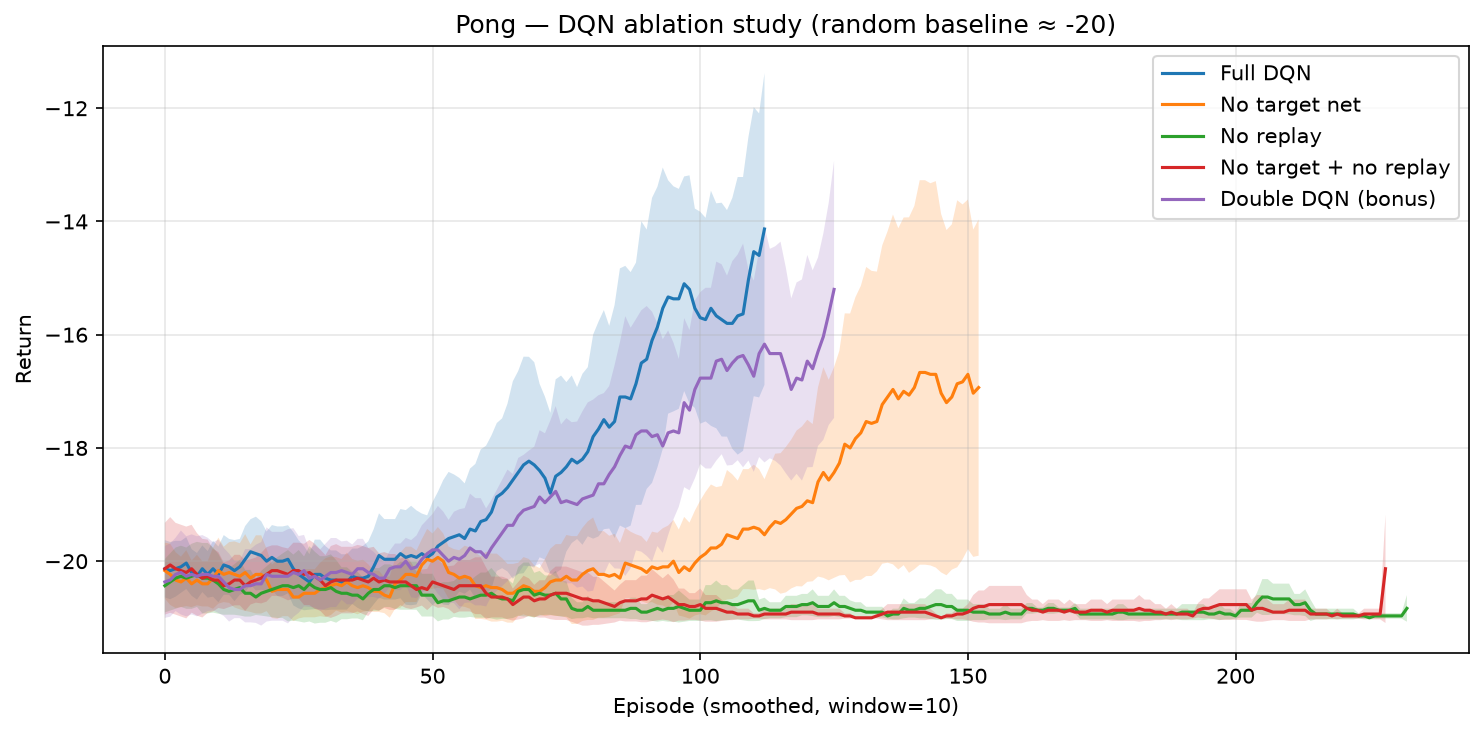
\includegraphics[width=0.55\linewidth]{pong_full_comparison.png}
\caption{Pong: ablazione DQN completa (200k step, 3 seed, baseline casuale
$\approx -20$). DQN completo (blu) e Double DQN (viola) apprendono; senza target network
(arancio) si impara pi\`u tardi e peggio; le due configurazioni senza replay (verde e
rosso) restano piatte al livello casuale.}
\label{fig:pong-full}
\end{figure}

\begin{figure}[htbp]
\centering
\begin{subfigure}{0.46\linewidth}
  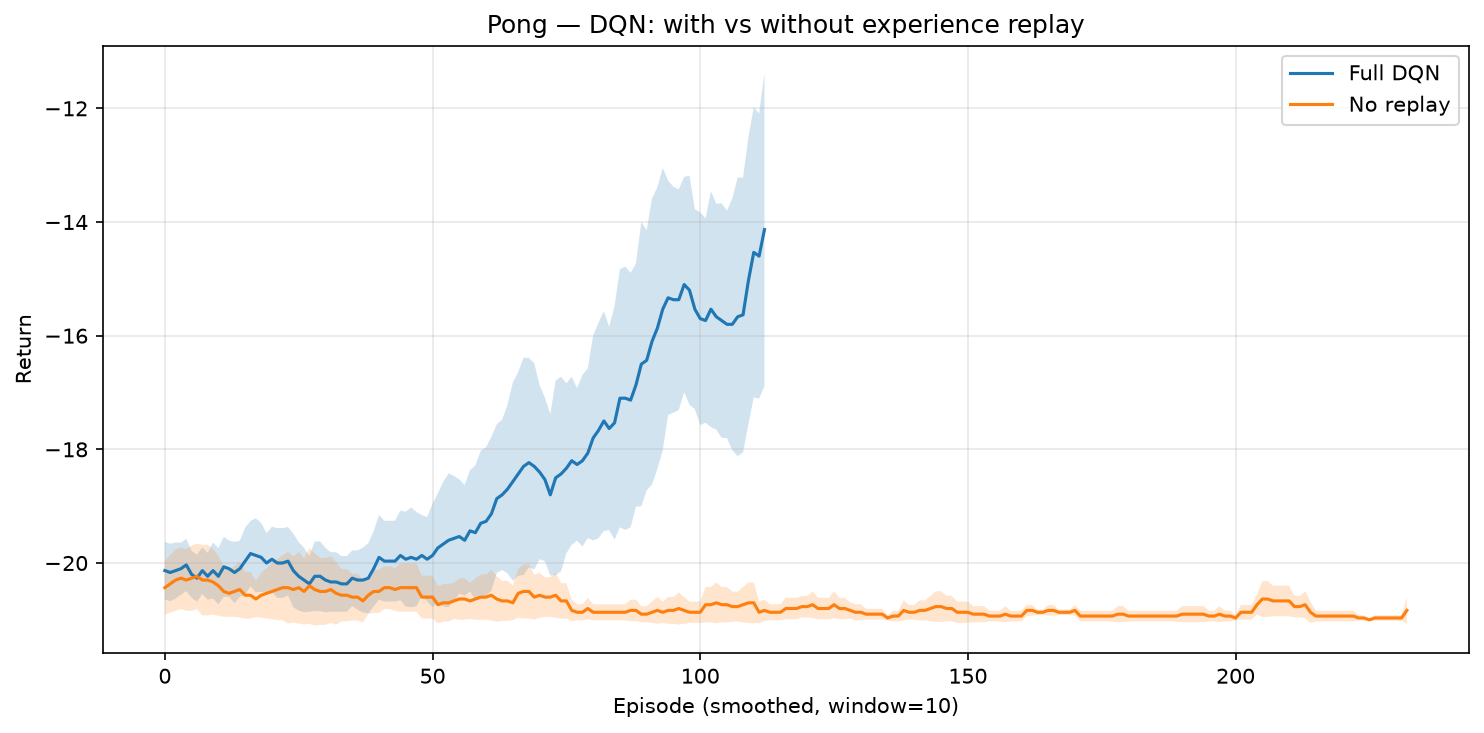
\includegraphics[width=\linewidth]{pong_ablation_replay.png}
  \caption{Con vs senza experience replay.}
\end{subfigure}\hfill
\begin{subfigure}{0.46\linewidth}
  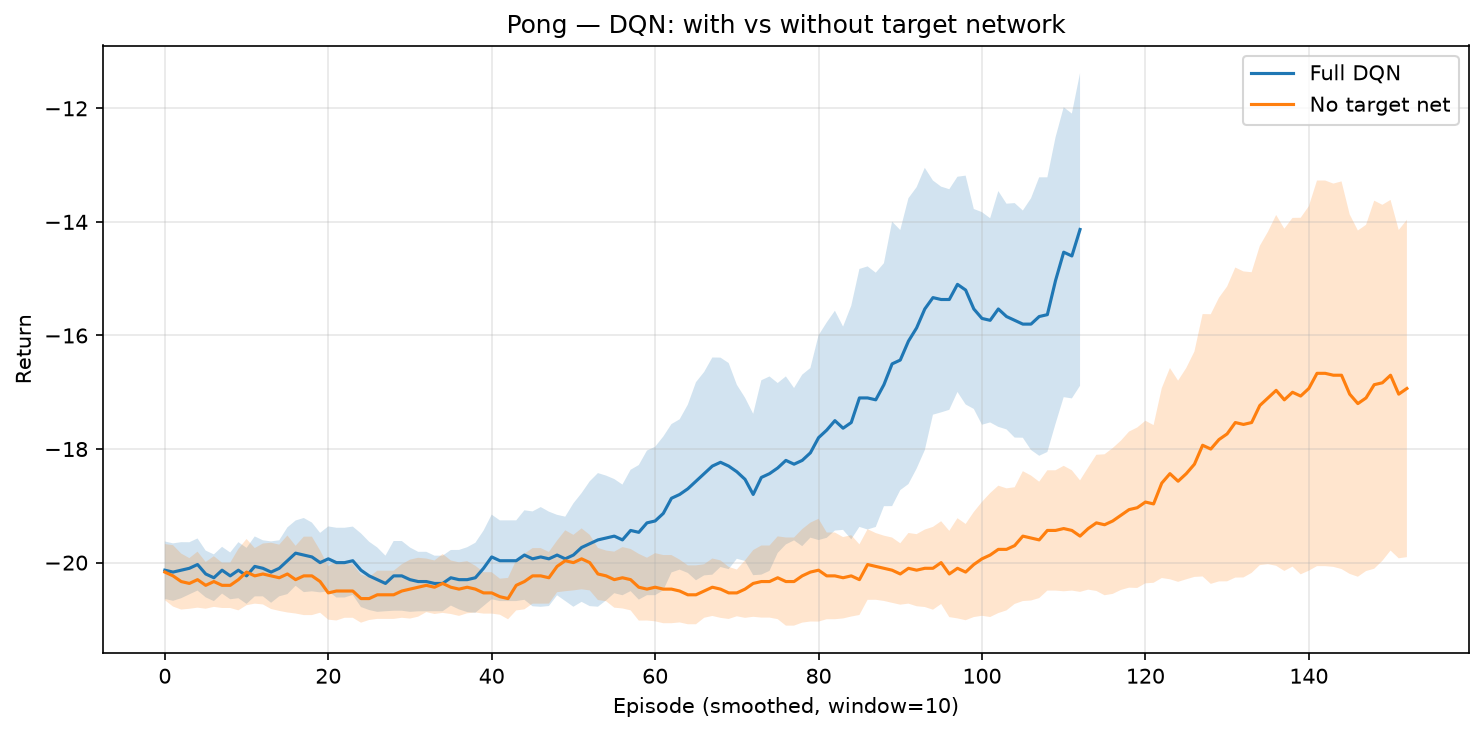
\includegraphics[width=\linewidth]{pong_ablation_target.png}
  \caption{Con vs senza target network.}
\end{subfigure}
\caption{Pong: le due ablazioni richieste dalla consegna, isolate. (a) Senza replay la
curva non si stacca mai dal livello casuale: componente \emph{necessario}. (b) Senza
target network l'apprendimento avviene, ma pi\`u tardi e con banda $\pm1\sigma$ molto
pi\`u larga: componente \emph{stabilizzante}.}
\label{fig:pong-ablation}
\end{figure}

\begin{table}[htbp]
\centering
\caption{Ablazione DQN su Pong: performance finale dopo 200k step ambiente, media $\pm$ std su 3 seed. Policy casuale $\approx -20.4$.}
\label{tab:pong-ablation}
\begin{tabular}{lcc}
\toprule
Configurazione & Return finale & Episodi/seed \\
               & (ultimo 10\% ep, media $\pm$ std) & (media) \\
\midrule
DQN completo (replay + target) & $-12.1 \pm 0.9$ & 134 \\
Double DQN (bonus) & $-14.2 \pm 0.8$ & 154 \\
Senza target network & $-16.3 \pm 2.8$ & 187 \\
Senza experience replay & $-20.6 \pm 0.2$ & 243 \\
Senza target + senza replay & $-20.5 \pm 0.3$ & 238 \\
\bottomrule
\end{tabular}
\end{table}


\section{Analisi critica}
\label{sec:discussion}

Questa sezione raccoglie le letture \emph{trasversali}, che nessun singolo esperimento
mostra da solo.

\subsection{SARSA vs Q-Learning: la teoria non predice il vincitore}
Il confronto ha prodotto esiti \emph{opposti} nei due ambienti, ed \`e istruttivo
proprio per questo. Su \textbf{CartPole} SARSA prevale su entrambi i fronti (return
$258$ vs $224$, deviazione standard $\pm 31$ vs $\pm 49$), mentre su \textbf{Acrobot}
Q\hbox{-}Learning ottiene un return leggermente migliore ($-341$ vs $-349$) ma SARSA
risulta quasi dieci volte pi\`u stabile tra i seed ($\pm 3.2$ vs $\pm 27.8$).

La differenza teorica \`e sempre la medesima: il target di Q\hbox{-}Learning impiega il
$\max$ e ignora l'esplorazione, quello di SARSA impiega l'azione realmente scelta e la
include. Le \emph{conseguenze}, tuttavia, dipendono dall'ambiente. L\`a dove
l'esplorazione \`e rischiosa (CartPole: una mossa casuale pu\`o far cadere l'asta),
SARSA guadagna perch\'e apprende una policy robusta al proprio rumore esplorativo. L\`a
dove il reward \`e sparso (Acrobot), il $\max$ di Q\hbox{-}Learning amplifica le rare
traiettorie fortunate che raggiungono l'obiettivo: quali siano dipende dal seed, il che
spiega i picchi pi\`u elevati ma anche la varianza molto superiore. Concludere che
``off-policy \`e meglio'' non ha pertanto valore predittivo: ci\`o che conta \`e come il
rischio dell'esplorazione interagisce con la struttura del reward.

\subsection{Perch\'e le curve non convergono mai davvero}
Nessuna curva tabellare si appiattisce del tutto, in lincea con le previsioni: con $\varepsilon$ e
$\alpha$ \emph{costanti} l'agente continua a esplorare e dunque la fluttuazione
asintotica \`e un comportamento atteso (S\&B \S2.5). Il fatto che l'annealing di
$\varepsilon$ riduca sensibilmente la varianza tra seed su entrambi gli ambienti ne
costituisce la conferma sperimentale (almeno funo a quanto il valore di $\varepsilon$ non si fissa nuovamente).

\subsection{Limiti metodologici riconosciuti}
\begin{itemize}
  \item \textbf{Predizione: misura locale.} Il confronto MC vs TD(0) traccia
        $V(s_{\text{ref}})$ di \emph{un} singolo stato; una misura globale (RMSE di $V$
        su tutti gli stati, come nel \emph{random walk} del corso) richiederebbe un $V$
        di riferimento (il ground truth) che in questi ambienti non \`e disponibile a causa della struttura
        del problema, con un numero finito di stati da valutare.
  \item \textbf{Asse x in ``episodi'' nell'ablazione Pong.} A parit\`a di 200k step le
        diverse configurazioni producono numeri diversi di episodi, per cui confrontarle
        allo stesso indice non costituisce un confronto a perfetta parit\`a di calcolo. Un
        asse in step ambiente sarebbe pi\`u rigoroso; la conclusione qualitativa non
        cambia, dal momento che le curve senza replay restano piatte per l'intera durata.
  \item \textbf{Bande assenti nelle figure di sensibilit\`a}, per ragioni di
        leggibilit\`a (Sez.~\ref{sec:experiments-reading}).
  \item \textbf{Il DQN \`e valutato durante il training}, con $\varepsilon > 0$: si
        tratta di una stima leggermente \emph{pessimistica} della policy greedy. I
        checkpoint sono salvati, e una valutazione greedy separata sarebbe fattibile senza
        necessit\`a di riaddestrare.
\end{itemize}

\subsection{Problemi implementativi incontrati}
Distinti dai limiti intrinseci del RL, questi sono ostacoli concreti che \`e stato
necessario risolvere:
\begin{itemize}
  \item \textbf{GPU Blackwell (RTX 5060)}: richiede la build PyTorch CUDA 12.8; con
        build precedenti la GPU non viene rilevata e il training ricade silenziosamente
        su CPU.
  \item \textbf{Pipeline Atari, tre insidie}: (i) l'ambiente \code{-v5} possiede gi\`a
        un frame-skip interno che, combinato con \code{AtariPreprocessing}, produrrebbe
        uno skip effettivo di 16 frame, rendendo necessario forzare
        \code{frameskip=1}; (ii) in Gymnasium 1.x \code{FrameStack} si chiama
        \code{FrameStackObservation}; (iii) i frame impilati sono gi\`a in formato
        channel-first \code{(4,84,84)} e non devono essere trasposti. Un errore su uno
        qualsiasi dei tre produce un crash oppure, peggio ancora, input silenziosamente
        malformati.
  \item \textbf{Memoria del replay buffer}: 1M di transizioni Atari
        richiederebbero $\approx 28$\,GB, pertanto il buffer \`e stato limitato a 100k
        transizioni mantenendo i frame in formato \code{uint8}.
  \item \textbf{DQN non riproducibile per un RNG nascosto.} Run che avrebbero dovuto
        essere identiche divergevano: l'azione esplorativa viene estratta da
        \code{env.action\_space.sample()}, e lo spazio delle azioni dispone di un
        \emph{RNG separato} che n\'e \code{set\_seed} n\'e \code{reset(seed=)}
        inizializzano. Nelle fasi iniziali ($\varepsilon\!\approx\!1$) quasi tutta
        l'esperienza proveniva da quel RNG non seminato. Aggiunto
        \code{env.action\_space.seed(seed)}; i risultati Pong riportati provengono da
        questo run corretto e riproducibile.
  \item \textbf{Episodio troncato contato come completo.} In DQN, quando il budget di step si
        esauriva a met\`a partita, il return parziale (troppo ottimistico) veniva
        registrato come episodio completo, producendo un picco spurio verso l'alto sul
        bordo destro di ogni curva. Corretto scartando l'episodio non terminato.
\end{itemize}

\section{Analisi sperimentale e lezioni apprese}
\label{sec:lessons}

Questa sezione documenta il \emph{processo} sperimentale, non solo i risultati
finali: cosa ci si aspettava, cosa ha funzionato, cosa no, quali problemi sono
emersi durante lo sviluppo e quali correzioni sono state applicate. L'obiettivo
\`e una discussione onesta, con ogni affermazione ancorata all'evidenza
sperimentale (Sez.~\ref{sec:results}).

\subsection{Obiettivi iniziali di ciascun esperimento}
\begin{itemize}[nosep]
  \item \textbf{CartPole controllo}: verificare che i metodi tabellari
        apprendano davvero e confrontare on-policy (SARSA) vs off-policy
        (Q\hbox{-}Learning).
  \item \textbf{Sensibilit\`a} ($\varepsilon,\alpha,\gamma$): mostrare l'effetto
        degli iperparametri sulla velocit\`a e stabilit\`a dell'apprendimento.
  \item \textbf{MC vs TD(0)}: illustrare il compromesso bias/varianza tra i due
        stimatori di predizione.
  \item \textbf{Casi di fallimento}: rendere visibili instabilit\`a
        ($\alpha$ estremo) e mancata esplorazione ($\varepsilon=0$).
  \item \textbf{Acrobot}: applicare gli stessi metodi a un ambiente pi\`u
        difficile (reward sparso, stato 6-D) e discutere i limiti della
        discretizzazione.
  \item \textbf{Pong/DQN}: implementare un DQN da zero e isolare, per ablazione,
        il contributo di experience replay e target network; testare Double DQN.
\end{itemize}

\subsection{Cosa ha funzionato}
\begin{itemize}[nosep]
  \item \textbf{Apprendimento tabellare corretto}: su CartPole entrambi gli
        algoritmi salgono da $\sim$30 fino a $\sim$175--225 (ancora in salita a
        5000 episodi dopo il fix \#2); Q\hbox{-}Learning mostra varianza tra seed
        pi\`u bassa (Tab.~\ref{tab:cartpole-control}).
  \item \textbf{Sensibilit\`a coerente con la teoria}: $\alpha=0.1$ \`e il
        compromesso migliore, $\gamma$ alto vince su un compito di
        sopravvivenza (Sez.~\ref{sec:res-cartpole-sens}).
  \item \textbf{Casi di fallimento riproducibili}: $\alpha=1.0$ e
        $\varepsilon=0$ producono i fallimenti attesi
        (Sez.~\ref{sec:res-cartpole-fail}).
  \item \textbf{Ablazione DQN da manuale}: replay indispensabile, target network
        acceleratrice; risultato netto e riproducibile
        (Fig.~\ref{fig:pong}, Tab.~\ref{tab:pong-ablation}).
  \item \textbf{Riproducibilit\`a}: media su 3 seed con bande, seeding combinato
        (numpy+torch+env), array grezzi salvati in \code{.npz} e tabelle
        generate da quei dati.
  \item \textbf{Bonus Double DQN}: implementato e funzionante (apprende in modo
        simile al DQN completo).
\end{itemize}

\subsection{Cosa non ha funzionato (o ha sorpreso)}
\begin{itemize}[nosep]
  \item \textbf{Il grafico MC vs TD(0) iniziale era poco informativo}: mostrava
        curve identiche, perch\'e tracciava il return della policy condivisa e
        non le stime $V(s)$. Corretto (fix \#1, Sez.~\ref{sec:lessons-fixes}).
  \item \textbf{Due ipotesi su Acrobot smentite dai dati}: bin pi\`u fini sono
        risultati \emph{migliori} (non peggiori) e $\varepsilon$ basso batte
        $\varepsilon$ alto (Sez.~\ref{sec:res-acrobot-bins},
        \ref{sec:res-acrobot-eps}). Risultati mantenuti e analizzati, non
        ``aggiustati''.
  \item \textbf{CartPole non raggiungeva 500} ma si fermava a $\sim$184: un
        \emph{tetto di discretizzazione}, non un bug. Il fix \#2 lo ha alzato
        ($\sim$225) ma al prezzo di convergenza pi\`u lenta e varianza maggiore
        --- un miglioramento \emph{a doppio taglio}, non netto (vedi
        Sez.~\ref{sec:lessons-fixes}).
  \item \textbf{Acrobot lontano dall'ottimo} ($\sim$$-345$ vs $\sim$$-100$) e con
        curve molto rumorose: atteso per reward sparso e spazio grande.
  \item \textbf{Double DQN non supera il DQN base} nel regime breve (200k step):
        la riduzione del maximization bias non \`e determinante con cos\`i pochi
        step; comportamento noto in letteratura, non un errore.
\end{itemize}

\subsection{Problemi incontrati durante lo sviluppo}
\label{sec:lessons-problems}
Questi sono problemi \emph{implementativi} reali (distinti dai limiti
intrinseci dell'RL discussi sotto):
\begin{itemize}[nosep]
  \item \textbf{GPU Blackwell (RTX 5060)}: richiede la build PyTorch CUDA 12.8;
        con build pi\`u vecchie la GPU non viene rilevata.
  \item \textbf{Pipeline Atari, tre trappole risolte}: (i) l'ambiente
        \code{-v5} ha gi\`a un frame-skip interno, che combinato con
        \code{AtariPreprocessing} darebbe uno skip di 16 frame $\Rightarrow$ si
        forza \code{frameskip=1} alla creazione; (ii) in Gymnasium 1.x
        \code{FrameStack} \`e stato rinominato \code{FrameStackObservation};
        (iii) i frame impilati arrivano gi\`a in formato channel-first
        \code{(4,84,84)}, quindi \emph{non} va applicata alcuna trasposizione
        prima della CNN. Un errore su uno qualsiasi di questi tre punti produce
        crash o input malformati alla rete.
  \item \textbf{Registrazione ALE}: con \code{ale-py} recente serve
        \code{gym.register\_envs(ale\_py)}, altrimenti \code{gym.make("ALE/...")}
        fallisce.
  \item \textbf{Memoria del replay buffer}: 1M transizioni Atari a frame interi
        sarebbero $\sim$28\,GB; si \`e limitato il buffer a 100k transizioni e si
        conservano i frame in \code{uint8}, normalizzando solo al training.
  \item \textbf{Backend Matplotlib}: forzato ad \code{Agg} (non interattivo) per
        salvare le figure senza GUI.
  \item \textbf{Conflitti di versione nel codice}: durante la gestione con
        \code{git} sono rimasti dei marcatori di merge non risolti in alcuni file
        (Atari/DQN/plotting). Sono stati risolti mantenendo la versione
        \emph{effettivamente eseguita} (quella che ha prodotto i risultati Pong),
        e verificati con un test di import dell'intero pacchetto.
\end{itemize}

\subsection{Correzioni applicate}
\label{sec:lessons-fixes}
\paragraph{Fix \#1 --- confronto MC vs TD(0) reso significativo.}
\emph{Cosa}: oltre al return della policy, si traccia ora la stima
$V(s_{\text{ref}})$ di uno stato di riferimento episodio per episodio.
\emph{Perch\'e}: il return \`e identico per costruzione tra i due metodi (stessa
policy), quindi non pu\`o mostrare la differenza; la differenza bias/varianza
vive nelle stime $V$.
\emph{Effetto}: su CartPole la stima MC salta rapidamente al valore corretto
($\sim$90 sulla policy appresa) con alta varianza iniziale, mentre TD(0) parte
da 0 e sale lentamente (distorsione da bootstrap) in modo liscio --- il quadro
classico di Sutton \& Barto \S6.2 (Fig.~\ref{fig:pred-value}).
\emph{Un bug scoperto e corretto durante questa verifica}: la prima scelta dello
stato di riferimento era il ``bin centrale'' su ogni dimensione. Su Acrobot ci\`o
d\`a uno stato \emph{fisicamente impossibile} --- l'osservazione codifica gli
angoli come $[\cos\theta, \sin\theta,\dots]$ e $\cos\theta,\sin\theta$ non
possono essere entrambi $\approx 0$ --- quindi quello stato non viene mai
visitato e la stima restava piatta a $0$. Corretto usando lo \emph{stato di
reset discretizzato}, sempre raggiungibile e visitato ad ogni episodio
(Fig.~\ref{fig:ac-pred-value}).
\emph{Risolto?} S\`i, entro l'approccio scelto (un singolo stato di
riferimento); una misura globale (RMSE di $V$ su tutti gli stati) richiederebbe
un $V$ di riferimento non disponibile qui.

\paragraph{Fix \#2 --- discretizzazione CartPole pi\`u efficiente.}
\emph{Cosa}: gli intervalli di clipping di posizione e angolo sono stati
ristretti dai limiti dello spazio di osservazione ($\pm4.8$, $\pm0.418$) ai
limiti di \emph{terminazione} ($\pm2.4$, $\pm0.21$).
\emph{Perch\'e}: oltre i limiti di terminazione l'episodio \`e gi\`a finito,
quindi met\`a dei bin di posizione e angolo era sprecata su stati che non
possono verificarsi.
\emph{Effetto (a doppio taglio, non netto)}: raddoppia la risoluzione utile sulle
due dimensioni pi\`u importanti e \emph{alza il tetto} --- le curve superano il
vecchio plateau di $\sim$184 e SARSA arriva a $\sim$225. Ma pi\`u stati
significano convergenza \emph{pi\`u lenta} (curve ancora in salita a 5000
episodi) e \emph{varianza maggiore} tra seed ($\pm 39$/$\pm 61$ contro
$\pm 8$/$\pm 18$). Inoltre l'ordine cambia: SARSA ora supera Q\hbox{-}Learning
(Tab.~\ref{tab:cartpole-control}).
\emph{Risolto?} Il ``tetto'' si alza ma non sparisce: resta un limite di ogni
metodo tabellare su stato continuo (serve approssimazione di funzione).

\subsection{Limiti residui}
\label{sec:lessons-limits}
Alcuni limiti restano anche dopo le correzioni. \`E importante distinguere quelli
\emph{intrinseci all'RL} da eventuali difetti di implementazione: i seguenti sono
caratteristiche attese, non bug.
\begin{itemize}[nosep]
  \item \textbf{Efficienza campionaria (sample efficiency) bassa}: i metodi
        tabellari richiedono migliaia di episodi (5k CartPole, 10k Acrobot) per
        risultati modesti. \`E inerente al tabular senza generalizzazione.
  \item \textbf{Stabilit\`a di convergenza}: le curve non si appiattiscono mai del
        tutto. Con $\varepsilon$ e $\alpha$ \emph{costanti}, l'agente continua a
        esplorare e pesa le esperienze recenti in modo esponenziale: la
        fluttuazione asintotica \`e attesa, non un errore.
  \item \textbf{Sparsit\`a del reward (Acrobot)}: reward $-1$/passo fino
        all'obiettivo rende l'assegnazione del credito difficile; spiega la
        convergenza lenta e la distanza dall'ottimo.
  \item \textbf{Sensibilit\`a agli iperparametri}: i risultati dipendono
        marcatamente da $\alpha,\gamma,\varepsilon$ e dal numero di bin (Sez.~
        \ref{sec:res-cartpole-sens}, \ref{sec:res-acrobot-bins}). Tipico dell'RL.
  \item \textbf{Varianza da seed / casualit\`a}: le bande $\pm1\sigma$ sono a
        volte ampie (Acrobot, predizione). Con solo 3 seed la stima
        dell'incertezza \`e essa stessa rumorosa; \`e un compromesso di budget,
        dichiarato apertamente.
  \item \textbf{Vincoli computazionali (Pong)}: 200k step contro i 50M del paper
        Nature; per questo Pong si ferma a $\sim$$-12$ e non a punteggi positivi.
        \`E una scelta di budget, non un difetto dell'implementazione.
  \item \textbf{Strategia di esplorazione}: $\varepsilon$-greedy costante \`e la
        pi\`u semplice; su Acrobot un valore alto \emph{costante} penalizza
        (Sez.~\ref{sec:res-acrobot-eps}). Un annealing sarebbe pi\`u adatto.
  \item \textbf{Generalizzazione / discretizzazione}: la discretizzazione
        uniforme perde precisione (tetto di CartPole; Acrobot lontano
        dall'ottimo). Non \`e overfitting in senso classico ma
        \emph{sotto-rappresentazione} dello stato: il limite \`e la griglia, non
        i dati.
  \item \textbf{Predizione, misura locale}: il fix \#1 mostra la varianza su
        \emph{un} stato di riferimento, non l'errore globale su $V$.
\end{itemize}

\subsection{Possibili miglioramenti futuri}
\label{sec:lessons-future}
Realistici, oltre gli obiettivi del corso:
\begin{itemize}[nosep]
  \item \textbf{Annealing di $\varepsilon$ e decadimento di $\alpha$}: curve pi\`u
        pulite e migliore convergenza asintotica.
  \item \textbf{Approssimazione di funzione per Acrobot}: tile coding o una
        piccola rete al posto della tabella, per superare la maledizione della
        dimensionalit\`a.
  \item \textbf{DQN pi\`u lungo e varianti}: pi\`u step, pi\`u Dueling DQN e
        Prioritized Experience Replay, verso punteggi positivi su Pong.
  \item \textbf{Predizione pi\`u rigorosa}: RMSE di $V$ rispetto a un riferimento
        Monte Carlo ad alta campionatura, come nell'esercizio \code{random\_walk}.
  \item \textbf{Ablazione Pong in funzione degli step ambiente}: confronto a
        parit\`a esatta di calcolo.
  \item \textbf{Fase di valutazione puramente greedy per il DQN}: separare il
        return di training (con esplorazione) da quello della policy finale.
\end{itemize}

\section{Conformit\`a alla consegna}
\label{sec:compliance}

La Tab.~\ref{tab:compliance} mappa ogni requisito della consegna sul relativo
deliverable. Legenda stato: \checkmark{} soddisfatto, \textasciitilde{}
parziale.

\begin{table}[H]
\centering
\small
\caption{Matrice di conformit\`a requisiti $\to$ implementazione.}
\label{tab:compliance}
\begin{tabular}{p{6.6cm}cp{5.2cm}}
\toprule
Requisito & Stato & Evidenza \\
\midrule
\multicolumn{3}{l}{\textit{Env 1 --- CartPole (comune)}} \\
Q\hbox{-}Learning, SARSA, MC, TD(0) ``from scratch'' & \checkmark &
  \code{rl\_lab/algorithms/tabular/} \\
Discretizzazione stato continuo & \checkmark &
  \code{envs/discretizer.py}; Tab.~\ref{tab:envs} \\
Curve di apprendimento (reward vs episodi) & \checkmark &
  Fig.~\ref{fig:cp-control} \\
Sensibilit\`a a $\varepsilon,\alpha,\gamma$ & \checkmark &
  Sez.~\ref{sec:res-cartpole-sens}, 6 figure \\
SARSA vs Q\hbox{-}Learning (empirico + teorico) & \checkmark &
  Sez.~\ref{sec:res-cartpole-control}, \ref{sec:theory} \\
MC vs TD(0) (bias/varianza/stabilit\`a) & \checkmark &
  Fig.~\ref{fig:pred-value} (stima $V$); vedi fix \#1 in Sez.~\ref{sec:lessons-fixes} \\
$\geq 1$ caso di fallimento & \checkmark &
  Sez.~\ref{sec:res-cartpole-fail}, 2 casi \\
\midrule
\multicolumn{3}{l}{\textit{Env 2 --- Acrobot (assegnato)}} \\
Stessi algoritmi applicati & \checkmark &
  \code{run\_acrobot.py} \\
Difficolt\`a di esplorazione (reward sparso) & \checkmark &
  Sez.~\ref{sec:res-acrobot-eps} \\
Necessit\`a di discretizzazione/approssimazione & \checkmark &
  Sez.~\ref{sec:res-acrobot-bins} (esperimento sui bin) \\
\midrule
\multicolumn{3}{l}{\textit{Env 3 --- Pong (Atari, assegnato)}} \\
DQN ``from scratch'' (replay + target) & \checkmark &
  \code{algorithms/deep/dqn.py} \\
Ablazione con/senza target network & \checkmark &
  Fig.~\ref{fig:pong}, Tab.~\ref{tab:pong-ablation} \\
Ablazione con/senza experience replay & \checkmark &
  Fig.~\ref{fig:pong}, Tab.~\ref{tab:pong-ablation} \\
Apprendimento vs policy casuale & \checkmark &
  baseline $\approx-20.4$; DQN $-12.1$ \\
Double DQN (bonus) & \checkmark &
  flag \code{use\_double\_dqn}; Sez.~\ref{sec:res-pong} \\
\midrule
\multicolumn{3}{l}{\textit{Requisiti trasversali}} \\
Media su 3 seed + deviazione standard & \checkmark &
  tutte le figure/tabelle \\
Riproducibilit\`a & \checkmark &
  seeding, \code{.npz}, \code{uv.lock} \\
No librerie RL di alto livello (Env 1/2) & \checkmark &
  core scritto a mano; SB3 non usato \\
Report 10--15 pagine, con failure analysis & \checkmark &
  questo documento (LaTeX) \\
\bottomrule
\end{tabular}
\end{table}

\paragraph{Nota sul confronto MC vs TD(0).}
In una prima versione questo era l'unico requisito solo parzialmente
soddisfatto: la visualizzazione mostrava il return della policy (identico per
costruzione) e non il compromesso bias/varianza. Con il fix \#1
(Sez.~\ref{sec:lessons-fixes}) si traccia ora anche la stima $V(s_{\text{ref}})$
episodio per episodio, che espone la varianza alta di MC contro la traiettoria
liscia di TD(0): il requisito \`e ora pienamente soddisfatto. Resta come
possibile estensione una misura globale (RMSE di $V$ su tutti gli stati).

\section{Origine del codice}
\label{sec:code-origin}

Per trasparenza si dichiara la provenienza di ogni componente. Il dettaglio
completo \`e in \code{docs/origine\_codice.md}; qui si riporta la sintesi.

\begin{table}[H]
\centering
\small
\caption{Origine dei moduli. \emph{Adattato} = derivato dal materiale del
corso; \emph{Nuovo} = scritto da zero per questo progetto;
\emph{Standard} = replica di architetture note (citate).}
\label{tab:origin}
\begin{tabular}{p{5.2cm}p{2.6cm}p{5.2cm}}
\toprule
Componente & Origine & Fonte / note \\
\midrule
Q\hbox{-}Learning, SARSA & Adattato &
  esercitazioni del corso (\code{control.py}); adattato all'API Gymnasium e
  agli stati discretizzati \\
MC prediction, TD(0) & Adattato &
  \code{prediction.py}, esercizio ``random walk'' \\
Policy $\varepsilon$-greedy & Adattato &
  \code{Esercitazione\_RL} \\
Discretizzatore & Nuovo &
  gli ambienti del corso erano gi\`a discreti \\
Preprocessing Atari & Adattato &
  \code{Tutorial\_Gymnasium}; wrapper Gymnasium (non SB3) \\
Replay buffer & Nuovo &
  concetto da Mnih~et~al.~\cite{mnih2015} \\
Rete Nature-CNN / MLP & Standard &
  architettura da~\cite{mnih2015}, implementazione PyTorch originale \\
Loop di training DQN & Nuovo &
  parte pi\`u originale; il corso forniva solo DQN basato su SB3 (vietato) \\
Double DQN & Nuovo &
  da~\cite{vanhasselt2016}, $\sim$5 righe sul DQN base \\
Runner multi-seed & Ispirato &
  pattern \code{run\_bias\_experiment} del corso \\
Plotting (bande $\pm\sigma$) & Nuovo (parz.\ adattato) &
  \code{moving\_average} dal corso; curve multi-seed nuove \\
Script per ambiente, tabelle & Nuovo &
  \code{scripts/} \\
\bottomrule
\end{tabular}
\end{table}

In sintesi: i \emph{quattro algoritmi tabellari} sono adattati dalle
esercitazioni; il \emph{DQN}, il discretizzatore, l'infrastruttura
multi-seed e tutti gli script sono \emph{scritti da zero}. Nessun codice
Stable-Baselines3 \`e usato nel core, come richiesto dalla consegna.

\section{Conclusioni}
\label{sec:conclusions}

Rispondo esplicitamente alle tre domande richieste dalla consegna.

\subsection{Cosa non ha funzionato}
\begin{itemize}
  \item \textbf{Acrobot non decolla}: plateau a $\approx -345$ contro un ottimo di
        $\approx -100$, e nessun miglioramento per 15\,000 episodi. Raddoppiare il
        budget non serve, perch\'e il limite \`e la risoluzione della Q-table
        (Sez.~\ref{sec:res-acrobot-control}).
  \item \textbf{CartPole non raggiunge 500}: con $10^4$ stati il tetto in 10\,000
        episodi \`e circa met\`a del massimo. Anche qui il vincolo \`e rappresentativo,
        non algoritmico.
  \item \textbf{I tre fallimenti indotti} (Sez.~\ref{sec:failure}): $\alpha=1.0$ non
        converge, $\varepsilon=0$ resta subottimale, $\gamma=0$ non pu\`o imparare
        affatto --- e in tutti e tre il codice gira correttamente.
  \item \textbf{Double DQN non supera il DQN base} a 200k step, anzi lo peggiora: il
        maximization bias che dovrebbe correggere non ha ancora avuto il tempo di
        accumularsi (Sez.~\ref{sec:res-pong}).
  \item \textbf{Il DQN non era riproducibile}: lo spazio delle azioni ha un RNG separato
        che n\'e \code{set\_seed} n\'e \code{reset(seed=)} toccano, e da l\`i viene ogni
        azione esplorativa; due run con lo stesso seed divergevano. Scoperto e corretto
        (Sez.~\ref{sec:discussion}).
  \item \textbf{Il mio primo confronto MC vs TD(0) non misurava nulla}: graficava il
        return della policy condivisa, identico per costruzione tra i due stimatori ---
        ``giusto'' e inutile (Sez.~\ref{sec:res-cartpole-pred}).
\end{itemize}

\subsection{Cosa mi ha sorpreso}
\begin{itemize}
  \item \textbf{Le due ipotesi smentite su Acrobot}: pi\`u bin sono \emph{meglio} (non
        peggio --- l'aliasing di una griglia grossolana domina la curse of dimensionality),
        e \emph{meno} esplorazione \`e meglio a $\varepsilon$ costante, salvo poi essere
        battuta dall'annealing: il problema non era ``quanta'' esplorazione ma ``quando''
        (Sez.~\ref{sec:res-acrobot-bins}, \ref{sec:res-acrobot-eps}).
  \item \textbf{SARSA batte Q\hbox{-}Learning su CartPole}, con varianza minore. Mi
        aspettavo il contrario; ma la curva misura la performance \emph{con
        l'esplorazione attiva}, e SARSA \`e l'unico dei due che ne tiene conto.
  \item \textbf{Il bias di TD(0) non \`e una costante}: sulla policy casuale (episodi
        corti) TD raggiunge MC, su quella appresa ($\approx 330$ passi) resta indietro del
        $13\%$ --- dipende dalla distanza temporale dal reward, che il \emph{random walk}
        del corso nasconde.
  \item \textbf{Senza target network l'apprendimento \`e una lotteria}: mi aspettavo un
        agente ``pi\`u lento'', ho trovato invece che 2 seed su 3 non decollano affatto e
        solo uno impara. La media ($-20$) nasconde il fenomeno, il per-seed lo rivela: la
        target network non accelera soltanto, rende l'apprendimento \emph{affidabile}
        (Sez.~\ref{sec:res-pong}).
\end{itemize}

\subsection{Limiti degli algoritmi}
\begin{itemize}
  \item \textbf{Discretizzazione} --- il collo di bottiglia dominante, e ha due lame:
        pochi bin non distinguono stati che richiedono azioni diverse, troppi bin fanno
        esplodere lo spazio. Nessuna scelta di bin risolve entrambi i problemi: serve
        l'approssimazione di funzione. \`E la motivazione empirica del DQN.
  \item \textbf{Efficienza campionaria e convergenza} --- migliaia di episodi per
        risultati modesti (nessuna generalizzazione tra stati simili), e con $\alpha$ ed
        $\varepsilon$ costanti la stima fluttua senza mai convergere davvero.
  \item \textbf{Sparsit\`a del reward} --- su Acrobot il segnale ($-1$ per passo) non
        dice \emph{quale} azione fosse sbagliata: il credit assignment su 500 passi \`e il
        problema vero, e nessuno dei quattro algoritmi tabellari lo affronta.
  \item \textbf{Sensibilit\`a agli iperparametri} --- marcata, e in modi che cambiano da
        ambiente ad ambiente e persino da algoritmo ad algoritmo ($\alpha$ alto danneggia
        SARSA ma non Q\hbox{-}Learning).
  \item \textbf{Costo del Deep RL} --- il DQN risolve la rappresentazione, ma 200k step
        sono lo $0.4\%$ del budget Nature: \`e per questo che Pong si ferma a
        $\approx -13$, e che senza target network met\`a dei seed non decolla.
\end{itemize}



\bibliographystyle{plain}
\bibliography{references}

\end{document}
